%%%%%%%%%%%%%%%%%%%%%%%%%%%%%%%%%%%%%%%%%%%%%%%%%%%%%%%%%%%%%%%%%%%%%%%%%%%%%
%  The Degree--Atomic Number Commensurability Index
%  Theory, extremal results and chemical applicability
%  Ali Berkan Bektas
%%%%%%%%%%%%%%%%%%%%%%%%%%%%%%%%%%%%%%%%%%%%%%%%%%%%%%%%%%%%%%%%%%%%%%%%%%%%%

\documentclass[11pt,a4paper]{article}

\usepackage[utf8]{inputenc}
\usepackage[T1]{fontenc}
\usepackage{amsmath}
\usepackage{amssymb}
\usepackage{amsthm}
\usepackage{booktabs}
\usepackage{graphicx}
\usepackage{tikz}
\usepackage{geometry}
\geometry{margin=2.6cm}
\usepackage[hidelinks]{hyperref}

\theoremstyle{plain}
\newtheorem{theorem}{Theorem}[section]
\newtheorem{proposition}[theorem]{Proposition}
\newtheorem{lemma}[theorem]{Lemma}
\newtheorem{corollary}[theorem]{Corollary}
\newtheorem{conjecture}[theorem]{Conjecture}
\theoremstyle{definition}
\newtheorem{definition}[theorem]{Definition}
\newtheorem{problem}[theorem]{Problem}
\theoremstyle{remark}
\newtheorem{remark}[theorem]{Remark}
\newtheorem{example}[theorem]{Example}

\newcommand{\CDZ}{\mathcal{C}_{DZ}}
\newcommand{\CDZhom}{\mathcal{C}_{DZ}^{\mathrm{hom}}}
\newcommand{\gcdd}{\operatorname{gcd}}
\newcommand{\lcmm}{\operatorname{lcm}}

\title{The Degree--Atomic Number Commensurability Index:\\
Theory, Extremal Results and Chemical Applicability}
\author{Ali Berkan Bekta\c{s}\thanks{ORCID: \href{https://orcid.org/0009-0003-9305-5587}{0009-0003-9305-5587}} \and \.{I}smail Naci Cang\"ul \and Yeliz Kara \c{S}en\\[4pt]
\small Department of Mathematics, Bursa Uluda\u{g} University, Bursa, T\"urkiye}
\date{\today}

\begin{document}

\maketitle

\begin{abstract}
We introduce and study the \emph{degree--atomic number commensurability index}
\[
  \CDZ(G) \;=\; \sum_{uv\in E(G)} \frac{\gcdd(a_u,a_v)}{\sqrt{a_u a_v}},
  \qquad a_u = d_u Z_u ,
\]
of a molecular graph $G$, where $d_u$ is the degree and $Z_u$ the atomic number
of the atom at the vertex $u$. Unlike the vertex-degree-based indices in current
use, $\CDZ$ is not a function of the degree sequence alone; its edge
contributions measure the arithmetic commensurability of the endpoint weights,
and we show that each contribution equals
$\sqrt{\gcdd(a_u,a_v)/\lcmm(a_u,a_v)}$.

On the theoretical side we prove that $\CDZ(G)\le m$ with equality exactly when
$d_uZ_u$ is constant; that on graphs whose atoms share a common atomic number
$\CDZ$ reduces to a purely degree-based invariant, independently of $Z$; the
two-sided comparisons $R(G)\le\CDZ(G)\le\Delta R(G)$ and
$GA(G)/\Delta\le\CDZ(G)\le GA(G)$ with their equality cases characterised, the
first by the arithmetic condition that adjacent degrees be coprime; the sharp
bounds $\sqrt{n-1}\le\CDZ(T)\le n-3+\sqrt2$ over trees, attained precisely by
the star and the path; closed forms on the standard graph families, including
$\CDZ(K_{x,y})=\gcdd(x,y)\sqrt{xy}$; and a degree-class representation whose
coefficients, unusually, fail to be monotone. We further conjecture that no
$\CDZ$-minimising tree contains an edge joining two vertices of equal degree,
verify this exhaustively, reduce the case of an edge of type $(3,3)$, by an
explicit five-case local analysis, to a purely existential statement that we
verify up to sixteen vertices, and exhibit a tree on twelve vertices which no
single-edge move improves although it is far from optimal, showing that the case
of degree-two edges cannot be settled by a strict-descent argument. An exact identity for the effect of subdividing an edge explains why
the minimisers on $6$, $8$, $11$ and $16$ vertices contain a vertex of degree
two, shows that trees with the same degree sequence can differ in $\CDZ$, and
shows that the minimisers do not form a chain under subdivision.

On the empirical side we assess $\CDZ$ against eleven established indices on the
standard testbeds. No correlation exceeds $0.87$ on trees or $0.76$ on the
decane isomers, below every one of the $55$ mutual correlations among those
eleven indices themselves, so $\CDZ$ is not a rescaling of any of them. It ties
the best classical indices in discriminative power on the alkane isomers, but
is outperformed by them on five of six thermodynamic properties of the octane
isomers -- an
outcome we trace to the homogeneous reduction, since those skeletons are pure
carbon. Where the atomic-number component can act, the gain is categorical: over
all trees on seven vertices labelled by C, N and O, the classical indices
separate $0.1\%$ of the $9894$ structures and $\CDZ$ separates $65.3\%$, a
factor of about $590$, which vanishes exactly when the atomic numbers are held
constant. We also report, as a limitation, that on measured solubility and
LogD data the \emph{ordering} $\CDZ$ assigns to true positional isomers is
statistically indistinguishable from chance.

\medskip\noindent
\textbf{Keywords.} topological index, vertex-degree-based index, greatest common
divisor, extremal graphs, chemical trees, QSPR, discriminative power.

\medskip\noindent
\textbf{AMS 2020 Subject Classification.} 05C09, 05C92, 05C90, 92E10.
\end{abstract}

%%%%%%%%%%%%%%%%%%%%%%%%%%%%%%%%%%%%%%%%%%%%%%%%%%%%%%%%%%%%%%%%%%%%%%%%%%%%%
\section{Introduction}
\label{sec:intro}

Let $G=(V,E)$ be the hydrogen-suppressed molecular graph of a compound: each
vertex $u\in V$ corresponds to a heavy atom, each edge $uv\in E$ to a covalent
bond between two heavy atoms. We write $n=|V|$, $m=|E|$, $d_u$ for the degree of
$u$, $\Delta$ for the maximum degree, $N(u)$ for the neighbourhood of $u$, and
$Z_u$ for the atomic number of the atom at $u$. All graphs are simple and, unless
stated otherwise, connected.

A \emph{vertex-degree-based} (VDB) topological index is a graph invariant of the
form
\begin{equation}
\label{eq:vdb}
  TI(G) \;=\; \sum_{uv\in E} f(d_u,d_v)
\end{equation}
for a symmetric function $f$. The family began with the Randi\'c index
$R(G)=\sum_{uv\in E}(d_ud_v)^{-1/2}$ \cite{randic1975} and the Zagreb indices
\cite{gutman1972,gutman1975}, and now includes the atom--bond connectivity index
$ABC$ \cite{estrada1998}, the geometric-arithmetic index $GA$
\cite{vukicevic2009}, the sum-connectivity indices $\chi_\alpha$
\cite{zhou2009}, the symmetric division deg index $SDD$ \cite{vukicevic2010},
and, more recently, the Sombor family \cite{gutman2021,liu2022} and the indices
obtained from the geometric picture of an edge developed by Gutman and
collaborators \cite{gutman2024,oz2025,furtula2025}, among them the tangent
Sombor index $Tan$ \cite{oz2025} and the geometric-quadratic index $GQ$
\cite{kulli2022,furtula2025ijmc}. A survey of the degree-based construction is
given by Gutman \cite{gutman2013} and the broader descriptor context by
Todeschini and Consonni \cite{todeschini2009}.

Two features of this literature motivate the present work.

First, every index of the form \eqref{eq:vdb} is a function of the degree
sequence and of nothing else. Consequently it assigns \emph{identical} values to
any two molecules whose hydrogen-suppressed graphs are isomorphic as abstract
graphs, however differently their heteroatoms are placed. The smallest instance
is ethanol (C--C--O) against dimethyl ether (C--O--C): both graphs are the path
$P_3$, so $R$, $ABC$, $M_1$, $M_2$, $SDD$, $SO$ and every other VDB index are
blind to the difference between an alcohol and an ether. This is not a defect of
any particular index but a structural consequence of the definition, and it is
not repaired by passing to a new function $f$.

Second, newly proposed VDB indices are now routinely found to be numerically
near-identical to existing ones. The correlation between $GQ$ and $GA$ on the
decane isomers is $0.99895$ \cite{furtula2025ijmc}, and between $Tan$ and the
inverse symmetric division deg index $0.99619$ \cite{oz2025}. Since all such
indices are linear functionals of the same edge-class vector, the family is
necessarily tightly inter-correlated, and a new member is of limited interest
unless it can be shown to carry information the others do not.

The index studied here addresses both points by leaving the class \eqref{eq:vdb}.
We attach to each vertex the composite weight $a_u=d_uZ_u$ and let each bond
contribute the ratio of the greatest common divisor of its endpoint weights to
their geometric mean. The resulting invariant depends on the \emph{arithmetic}
relation between the endpoint weights -- in a sense made precise in
Proposition~\ref{prop:lcm}, on how commensurable the two atoms are -- rather than
on their magnitudes, and it distinguishes heteroatom placement by construction.

The paper is organised as follows. Section~\ref{sec:def} fixes the definition and
establishes the basic structural facts, in particular the reduction
(Proposition~\ref{prop:homog}) of $\CDZ$ to a purely degree-based invariant on
graphs with a common atomic number; this reduction governs the interpretation of
every empirical result later in the paper. Section~\ref{sec:bounds} contains the
extremal theory: a general upper bound, two-sided comparisons with $R$ and $GA$,
sharp bounds for trees, the minimisation problem for chemical trees together with
a conjecture, an exact subdivision identity and a partial local analysis, and the
unicyclic case.
Section~\ref{sec:classes} records closed forms on the standard families and the
degree-class representation. Section~\ref{sec:empirical} is the empirical
assessment, following the protocol now standard in this literature
\cite{oz2025,furtula2025ijmc,kumar2024}: correlation with other indices,
correlation with physicochemical properties of the octane isomers,
discriminative power in the sense of Konstantinova \cite{konstantinova1996},
mutual correlation within the comparison set, structure sensitivity and
abruptness in the sense of Furtula, Gutman and Dehmer \cite{furtula2013}, and
finally the heteroatom tests that probe the one component no other VDB index
possesses. Section~\ref{sec:limits} delimits the applicability domain, reporting
in particular where the index fails. Section~\ref{sec:conclusion} concludes with
the open problems.

%%%%%%%%%%%%%%%%%%%%%%%%%%%%%%%%%%%%%%%%%%%%%%%%%%%%%%%%%%%%%%%%%%%%%%%%%%%%%
\section{Definition and basic properties}
\label{sec:def}

\begin{definition}[Degree--atomic number weight]
\label{def:weight}
For a vertex $u\in V(G)$ the \emph{degree--atomic number weight} of $u$ is
\[
  a_u \;=\; d_u\,Z_u .
\]
\end{definition}

\begin{definition}[Commensurability index]
\label{def:cdz}
The \emph{degree--atomic number commensurability index} of $G$ is
\[
  \boxed{\;
  \CDZ(G) \;=\; \sum_{uv\in E(G)} \frac{\gcdd(a_u,a_v)}{\sqrt{a_u\,a_v}}
  \;}
\]
where $\gcdd$ denotes the greatest common divisor of the two positive integers
$a_u$ and $a_v$.
\end{definition}

In a connected graph on $n\ge2$ vertices every vertex has $d_u\ge1$, hence
$a_u=d_uZ_u\ge1$ is a positive integer and every summand is well defined. For
$n=1$ the edge set is empty and we adopt the convention $\CDZ(K_1)=0$, so that a
single heavy atom such as methane receives the value $0$.

\begin{proposition}[Equivalent closed form]
\label{prop:lcm}
For every edge $uv\in E(G)$,
\[
  \frac{\gcdd(a_u,a_v)}{\sqrt{a_u a_v}}
  \;=\; \sqrt{\frac{\gcdd(a_u,a_v)}{\lcmm(a_u,a_v)}},
  \qquad\text{hence}\qquad
  \CDZ(G) \;=\; \sum_{uv\in E(G)}\sqrt{\frac{\gcdd(a_u,a_v)}{\lcmm(a_u,a_v)}} .
\]
\end{proposition}

\begin{proof}
For positive integers $a,b$ one has $ab=\gcdd(a,b)\lcmm(a,b)$. Writing
$g=\gcdd(a_u,a_v)$ and $\ell=\lcmm(a_u,a_v)$,
\[
  \frac{g}{\sqrt{a_ua_v}} \;=\; \frac{g}{\sqrt{g\ell}}
  \;=\; \sqrt{\frac{g^2}{g\ell}} \;=\; \sqrt{\frac{g}{\ell}},
\]
all quantities being positive, so the square roots are unambiguous.
\end{proof}

Proposition~\ref{prop:lcm} supplies the interpretation of the index: each bond
contributes the square root of the ratio of the greatest common divisor to the
least common multiple of its endpoint weights, that is, a normalised measure of
how \emph{arithmetically commensurable} the two atoms are. The contribution is
$1$ when the weights coincide and tends to $0$ as they become coprime and large.

\begin{proposition}[Range of the edge contribution]
\label{prop:range}
For every edge $uv$,
\[
  0 \;<\; \frac{\gcdd(a_u,a_v)}{\sqrt{a_ua_v}} \;\le\; 1,
\]
with equality on the right if and only if $a_u=a_v$.
\end{proposition}

\begin{proof}
Positivity is clear. Since $\gcdd(a_u,a_v)$ divides both arguments, we have
$\gcdd(a_u,a_v)\le\min\{a_u,a_v\}\le\sqrt{a_ua_v}$, the second step because the
smaller of two positive numbers cannot exceed their geometric mean; this gives
the upper bound. Equality forces
$\min\{a_u,a_v\}=\sqrt{a_ua_v}$, i.e.\ $a_u=a_v$; conversely if $a_u=a_v=a$ then
$\gcdd(a,a)/a=1$.
\end{proof}

\begin{proposition}[Reduction on homogeneous graphs]
\label{prop:homog}
Call $G$ \emph{homogeneous} if $Z_u=Z$ for every $u\in V$. For such a graph
\[
  \CDZ(G) \;=\; \sum_{uv\in E}\frac{\gcdd(d_u,d_v)}{\sqrt{d_ud_v}}
  \;=:\; \CDZhom(G),
\]
so $\CDZ$ becomes a purely degree-based invariant, independent of $Z$.
\end{proposition}

\begin{proof}
With $a_u=d_uZ$ and $a_v=d_vZ$ we have $\gcdd(d_uZ,d_vZ)=Z\gcdd(d_u,d_v)$ and
$\sqrt{a_ua_v}=Z\sqrt{d_ud_v}$; the factor $Z$ cancels.
\end{proof}

More generally the summand is unchanged under a simultaneous rescaling
$a_u\mapsto c\,a_u$ by a positive integer $c$: homogeneity of degree $0$ is
intrinsic to the construction, and Proposition~\ref{prop:homog} is its chemical
specialisation. We write $\CDZhom$ throughout for the invariant obtained by
setting $Z_u\equiv6$, i.e.\ by treating every atom as carbon; the difference
$\CDZ-\CDZhom$ isolates the contribution of the atomic numbers and will be used
repeatedly in Section~\ref{sec:empirical} as an ablation control.

\begin{remark}[Isomorphism invariance]
\label{rem:isom}
Both $d_u$ and $Z_u$ are preserved by any isomorphism of labelled molecular
graphs, and the summand depends on the unordered pair $\{a_u,a_v\}$ only; hence
$\CDZ$ is an invariant of the isomorphism class of the labelled graph. It is not
an invariant of the underlying unlabelled graph -- which is precisely the point
of the construction.
\end{remark}

\begin{remark}[Computational cost]
\label{rem:cost}
$\CDZ(G)$ is computed by one pass over the vertices, forming the weights
$a_u=d_uZ_u$, followed by one pass over the edges accumulating
$\gcdd(a_u,a_v)/\sqrt{a_ua_v}$, for a total running time of
$O(n+m\log Z_{\max})$. Since molecular graphs have bounded valence ($m=O(n)$)
and $Z_{\max}$ is a small constant, this is effectively linear in the size of
the molecule, and compares favourably with distance-based indices such as the
Wiener index, which require all pairwise shortest paths. In practice the cost of
evaluating $\CDZ$ is negligible beside that of parsing the input structure, as
confirmed on the library of $10\,833$ compounds used in
Section~\ref{sec:hetero}.
\end{remark}

\begin{remark}[Standing hypothesis]
\label{rem:standing}
Theorem~\ref{thm:general} below is stated for arbitrary weights $a_u=d_uZ_u$.
\emph{Every other result of Sections~\ref{sec:bounds} and~\ref{sec:classes}
assumes $G$ homogeneous}, so that Proposition~\ref{prop:homog} applies and
$\CDZ$ may be computed from the degrees alone. The hypothesis is not cosmetic.
Let $T=P_4$ carry the atomic numbers $(8,4,4,8)$ along the path; then
$(a_u)=(8,8,8,8)$, every edge contributes $1$ and $\CDZ(T)=3$, exceeding the
bound $n-3+\sqrt2\approx2.414$ of Theorem~\ref{thm:tree}. The tree bounds are
therefore genuinely statements about homogeneous graphs; chemically they apply
to hydrocarbon skeletons.
\end{remark}

%%%%%%%%%%%%%%%%%%%%%%%%%%%%%%%%%%%%%%%%%%%%%%%%%%%%%%%%%%%%%%%%%%%%%%%%%%%%%
\section{Extremal results and bounds}
\label{sec:bounds}

\subsection{A general upper bound}

\begin{theorem}[General upper bound]
\label{thm:general}
Let $G$ be a connected graph with $m$ edges, each vertex $u$ carrying the
positive integer weight $a_u=d_uZ_u$. Then
\[
  \CDZ(G)\;\le\; m,
\]
with equality if and only if $a_u=a_v$ for every $uv\in E$; since $G$ is
connected this is equivalent to the existence of a constant $c>0$ with
$d_uZ_u=c$ for all $u\in V$. In the homogeneous case equality holds if and only
if $G$ is regular.
\end{theorem}

\begin{proof}
By Proposition~\ref{prop:range} each summand is at most $1$, so
$\CDZ(G)\le m$. Equality in the sum forces equality in every summand, i.e.\
$a_u=a_v$ on every edge; connectivity propagates this along every path, giving
$a_u\equiv c$. If $Z_u\equiv Z$ then $d_uZ=d_vZ$ gives $d_u=d_v$ on every edge,
i.e.\ $G$ is regular.
\end{proof}

\subsection{Comparison with the Randi\'c index}

\begin{theorem}[Randi\'c sandwich]
\label{thm:randic}
Let $G$ be a homogeneous graph without isolated vertices and maximum degree
$\Delta$. Then
\[
  R(G) \;\le\; \CDZ(G) \;\le\; \Delta\,R(G).
\]
The left equality holds if and only if $\gcdd(d_u,d_v)=1$ for every $uv\in E$,
that is, adjacent vertices always have coprime degrees; the right equality holds
if and only if $G$ is regular.
\end{theorem}

\begin{proof}
On every edge $1\le\gcdd(d_u,d_v)\le\min\{d_u,d_v\}\le\Delta$. Dividing by
$\sqrt{d_ud_v}$ and summing over $E$ gives both inequalities. The left equality
requires $\gcdd(d_u,d_v)=1$ on every edge. The right requires
$\gcdd(d_u,d_v)=\Delta$ on every edge; since the gcd divides both $d_u$ and
$d_v$, and these are at most $\Delta$, this forces $d_u=d_v=\Delta$ on every
edge, i.e.\ $G$ is $\Delta$-regular. Conversely a $\Delta$-regular graph has
$\CDZ(G)=m$ and $\Delta R(G)=\Delta\cdot m/\Delta=m$.
\end{proof}

Theorem~\ref{thm:randic} is the sharpest expression of what separates $\CDZ$
from the indices in the literature. Relations between a new index and an
established one are usually approximate and statistical; here the relation is
exact and its equality case is characterised by a purely \emph{arithmetic}
condition on the degree sequence. In particular $\CDZ$ and $R$ coincide
identically on the class of graphs whose adjacent degrees are coprime, and
diverge exactly to the extent that adjacent degrees share common factors. The
following makes this quantitative.

\begin{definition}[$\CDZ$--Randi\'c gap]
\label{def:gap}
For a homogeneous graph $G$ without isolated vertices put
$\Gamma_{\CDZ}(G)=\CDZ(G)-R(G)$.
\end{definition}

\begin{proposition}
\label{prop:gap}
For every such $G$,
\[
  \Gamma_{\CDZ}(G) \;=\; \sum_{uv\in E}\frac{\gcdd(d_u,d_v)-1}{\sqrt{d_ud_v}}
  \;\ge\;0,
\]
with $\Gamma_{\CDZ}(G)=0$ if and only if $\gcdd(d_u,d_v)=1$ for every $uv\in E$.
Only edges with $\gcdd(d_u,d_v)>1$ contribute, so $\Gamma_{\CDZ}$ is supported
on the set of \emph{non-coprime} edges.
\end{proposition}

\begin{proof}
Subtract the two defining sums term by term. Each summand is nonnegative
because $\gcdd(d_u,d_v)\ge1$, and it vanishes exactly when this gcd equals $1$.
\end{proof}

\begin{corollary}[Sharp lower bound over connected graphs]
\label{cor:conn_lower}
Let $G$ be a homogeneous connected graph on $n\ge2$ vertices. Then
\[
  \CDZ(G)\;\ge\;\sqrt{n-1},
\]
with equality if and only if $G\cong S_n$.
\end{corollary}

\begin{proof}
By Theorem~\ref{thm:randic}, $\CDZ(G)\ge R(G)$, and by the theorem of
Bollob\'as and Erd\H{o}s \cite{bollobas1998} the Randi\'c index of a connected
graph on $n$ vertices satisfies $R(G)\ge\sqrt{n-1}$ with equality if and only if
$G\cong S_n$. Equality in the conclusion forces equality in both steps, and the
second already characterises the star. Conversely, in $S_n$ the centre has degree
$n-1$ and each leaf degree $1$; since $\gcdd(1,n-1)=1$, every edge contributes
$1/\sqrt{n-1}$, giving $\CDZ(S_n)=(n-1)/\sqrt{n-1}=\sqrt{n-1}=R(S_n)$.
\end{proof}

\begin{remark}
Corollary~\ref{cor:conn_lower} is stronger than the corresponding statement for
trees, holding over all connected graphs of order $n$; the star is
simultaneously the minimiser in both classes.
\end{remark}

\begin{remark}[The bound is vacuous for chemical trees with $n\ge6$]
\label{rem:chemical_gap}
Corollary~\ref{cor:conn_lower} minimises over \emph{all} trees on $n$ vertices,
and the minimiser $S_n$ has a vertex of degree $n-1$. For a \emph{chemical} tree
(maximum degree at most $4$, as carbon valence requires) such a vertex is
infeasible as soon as $n\ge6$, so $S_n$ does not lie in the class being
optimised over and the bound $\sqrt{n-1}$ is neither attained nor, numerically,
approached: for $n=6,\dots,13$ the true minimum over chemical trees is
$2.80806$, $2.94338$, $3.48138$, $3.88675$, $4.15470$, $4.69271$, $5.09808$,
$5.36603$, each well above $\sqrt{n-1}$. The sharp lower bound for chemical
trees is therefore a separate problem, taken up in
Section~\ref{sec:minimisers}.
\end{remark}

\begin{theorem}[Maximum-degree lower bound]
\label{thm:lower_delta}
Let $G$ be a homogeneous connected graph with $m$ edges and maximum degree
$\Delta$. Then $\CDZ(G)\ge m/\Delta$, with equality if and only if $G\cong K_2$.
\end{theorem}

\begin{proof}
On every edge $\gcdd(d_u,d_v)\ge1$ and $\sqrt{d_ud_v}\le\Delta$, so each summand
is at least $1/\Delta$. Equality in the sum requires $d_ud_v=\Delta^2$ on every
edge, hence $d_u=d_v=\Delta$, together with $\gcdd(\Delta,\Delta)=\Delta=1$;
thus $\Delta=1$ and $G\cong K_2$.
\end{proof}

\subsection{Comparison with the geometric-arithmetic index}

Let $GA(G)=\sum_{uv\in E}2\sqrt{d_ud_v}/(d_u+d_v)$ \cite{vukicevic2009}.

\begin{lemma}[Elementary inequality]
\label{lem:minmax}
For positive integers $a,b$,
\[
  \frac{\min\{a,b\}}{\sqrt{ab}}\;\le\;\frac{2\sqrt{ab}}{a+b},
\]
with equality if and only if $a=b$.
\end{lemma}

\begin{proof}
Both sides are positive, so after multiplying by the positive quantity
$\sqrt{ab}(a+b)$ the claim is equivalent to $\min\{a,b\}(a+b)\le2ab$. We show
\[
  2ab-\min\{a,b\}(a+b)\;=\;\min\{a,b\}\cdot|a-b|\;\ge\;0 .
\]
By symmetry assume $a\le b$, so $\min\{a,b\}=a$ and $|a-b|=b-a$; then
\[
  2ab-a(a+b) \;=\; ab-a^2 \;=\; a(b-a) \;=\; \min\{a,b\}\cdot|a-b| ,
\]
which is nonnegative. The product $\min\{a,b\}\cdot|a-b|$ vanishes exactly when
$a=b$, since the first factor is positive; this is therefore the equality case.
\end{proof}

\begin{theorem}[$GA$ sandwich]
\label{thm:ga}
Let $G$ be a homogeneous connected graph without isolated vertices and maximum
degree $\Delta$. Then
\[
  \frac{GA(G)}{\Delta}\;\le\;\CDZ(G)\;\le\;GA(G),
\]
with the right equality if and only if $G$ is regular.
\end{theorem}

\begin{proof}
\textbf{Upper bound.} Fix an edge $uv$. Since $\gcdd(d_u,d_v)$ never exceeds the
smaller of its two arguments, Lemma~\ref{lem:minmax} with $a=d_u$, $b=d_v$ gives
\[
  \frac{\gcdd(d_u,d_v)}{\sqrt{d_ud_v}}
  \;\le\;\frac{\min\{d_u,d_v\}}{\sqrt{d_ud_v}}
  \;\le\;\frac{2\sqrt{d_ud_v}}{d_u+d_v},
\]
whose right-hand side is the edge's contribution to $GA$. Summing over $E$ gives
$\CDZ(G)\le GA(G)$.

For equality every edge must attain equality in both steps. By
Lemma~\ref{lem:minmax} the second step is an equality precisely when $d_u=d_v$,
and in that case the first is automatic since
$\gcdd(d_u,d_u)=d_u=\min\{d_u,d_u\}$; if $d_u\ne d_v$ the second step is strict.
Hence equality on an edge holds if and only if $d_u=d_v$, and equality in the sum
requires this on every edge, which by connectivity propagates to $G$ regular.
Conversely a $\Delta$-regular graph has $\CDZ(G)=GA(G)=m$.

\textbf{Lower bound.} We chain three inequalities.

\emph{Step 1: $GA(G)\le m$.} For positive reals $x,y$ the arithmetic--geometric
mean inequality gives $2\sqrt{xy}\le x+y$, i.e.\ $2\sqrt{xy}/(x+y)\le1$;
applying this on each edge and summing over the $m$ edges yields $GA(G)\le m$.

\emph{Step 2: $m\le\Delta R(G)$.} On every edge $d_u,d_v\le\Delta$, so
$d_ud_v\le\Delta^2$ and $1/\sqrt{d_ud_v}\ge1/\Delta$; summing over the $m$ edges
gives $R(G)\ge m/\Delta$.

\emph{Step 3: $R(G)\le\CDZ(G)$.} This is the left inequality of
Theorem~\ref{thm:randic}.

Chaining, $GA(G)\le m\le\Delta R(G)\le\Delta\CDZ(G)$; divide by $\Delta$.
\end{proof}

\begin{remark}
Theorem~\ref{thm:ga} is the $\CDZ$ counterpart of the inequality
$GA(G)/\sqrt2<GQ(G)\le GA(G)$ established for the geometric-quadratic index in
\cite{furtula2025ijmc}. The mechanism differs: there the upper bound comes from
$2ab\le a^2+b^2$, here from $\gcdd(a,b)\le\min\{a,b\}$, so the bound reflects the
arithmetic origin of $\CDZ$ rather than a metric one.
\end{remark}

\subsection{Trees}
\label{sec:trees}

\begin{theorem}[Sharp upper bound for trees]
\label{thm:tree}
Let $T$ be a homogeneous tree on $n\ge3$ vertices. Then
\[
  \CDZ(T)\;\le\;n-3+\sqrt2,
\]
with equality if and only if $T\cong P_n$.
\end{theorem}

\begin{proof}
Let $\ell$ be the number of leaves; since $n\ge3$ we have $\ell\ge2$, distinct
leaves lie on distinct pendant edges, and the neighbour $v$ of a leaf satisfies
$d_v\ge2$. A pendant edge $uv$ with $d_u=1$ has $\gcdd(1,d_v)=1$ and so
contributes $1/\sqrt{d_v}\le1/\sqrt2$, while every other edge contributes at most
$1$ by Theorem~\ref{thm:general}. With $m=n-1$,
\[
  \CDZ(T)\;\le\;(m-\ell)+\frac{\ell}{\sqrt2}
  \;=\; m-\ell\Bigl(1-\tfrac1{\sqrt2}\Bigr)
  \;\le\;(n-1)-2\Bigl(1-\tfrac1{\sqrt2}\Bigr) \;=\; n-3+\sqrt2,
\]
the last step because $1-1/\sqrt2>0$ and $\ell\ge2$. Equality requires $\ell=2$,
hence $T\cong P_n$; that every pendant edge has $d_v=2$; and that every internal
edge joins equal degrees. All three hold in $P_n$, where the two pendant edges
contribute $1/\sqrt2$ each and the $n-3$ internal edges contribute $1$ each.
\end{proof}

\begin{theorem}[Complete extremal theorem for trees]
\label{thm:complete_tree}
For every homogeneous tree $T$ on $n\ge3$ vertices,
\[
  \boxed{\;\sqrt{n-1}\;\le\;\CDZ(T)\;\le\;n-3+\sqrt2\;}
\]
with the left equality if and only if $T\cong S_n$ and the right if and only if
$T\cong P_n$.
\end{theorem}

\begin{proof}
Combine Corollary~\ref{cor:conn_lower} with Theorem~\ref{thm:tree}.
\end{proof}

\begin{remark}
For $n=3$ the two bounds coincide, both equalling $\sqrt2$; this is consistent,
since $P_3\cong S_3$.
\end{remark}

\begin{corollary}
\label{cor:alkane_max}
Among all alkane isomers with $n$ carbon atoms the unbranched $n$-alkane
uniquely maximises $\CDZ$, with value $n-3+\sqrt2$.
\end{corollary}

\subsection{Minimising trees}
\label{sec:minimisers}

By Remark~\ref{rem:chemical_gap} the minimisation of $\CDZ$ over chemical trees
is not settled by Corollary~\ref{cor:conn_lower}, and it turns out to be
considerably harder than the maximisation. We record the computational evidence
and a structural conjecture; identify a two-parameter family that contains most
of the minimisers; prove an exact subdivision identity that explains the
remaining ones; and present a partial local analysis together with an
obstruction showing that this analysis cannot be completed by local means
alone.

Table~\ref{tab:minimisers} lists, for $4\le n\le17$, the minimum of $\CDZ$ over
all chemical trees on $n$ vertices, obtained by exhaustive enumeration.

\begin{table}[htbp]
\centering
\caption{Minimisers of $\CDZ$ over chemical trees on $n$ vertices. The column
``internal degrees'' describes each minimiser but does not determine it; see
Proposition~\ref{prop:432}.}
\label{tab:minimisers}
\begin{tabular}{rlll}
\toprule
$n$ & $\min\CDZ$ & internal degrees & edge types present \\
\midrule
$4$  & $1.7321$ & $[3]$           & $(1,3)$ \\
$5$  & $2.0000$ & $[4]$           & $(1,4)$ \\
$6$  & $2.8081$ & $[3,2,2]$       & $(1,2),(1,3),(2,3)$ \\
$7$  & $2.9434$ & $[4,3]$         & $(1,3),(1,4),(3,4)$ \\
$8$  & $3.4814$ & $[4,3,2]$       & $(1,2),(1,3),(1,4),(2,3),(3,4)$ \\
$9$  & $3.8868$ & $[4,3,3]$       & $(1,3),(1,4),(3,4)$ \\
$10$ & $4.1547$ & $[4,4,3]$       & $(1,3),(1,4),(3,4)$ \\
$11$ & $4.6927$ & $[4,4,3,2]$     & $(1,2),(1,4),(2,3),(3,4)$ \\
$12$ & $5.0981$ & $[4,4,3,3]$     & $(1,3),(1,4),(3,4)$ \\
$13$ & $5.3660$ & $[4,4,4,3]$     & $(1,4),(3,4)$ \\
$14$ & $6.0415$ & $[4,4,3,3,3]$   & $(1,3),(1,4),(3,4)$ \\
$15$ & $6.3094$ & $[4,4,4,3,3]$   & $(1,3),(1,4),(3,4)$ \\
$16$ & $6.7599$ & $[4,4,4,3,3,2]$ & $(1,3),(1,4),(2,3),(3,4)$ \\
$17$ & $7.2528$ & $[4,4,4,3,3,3]$ & $(1,3),(1,4),(3,4)$ \\
\bottomrule
\end{tabular}
\end{table}

In none of these fourteen cases does the minimiser contain an edge whose two
endpoints have equal degree. This is exactly what
Proposition~\ref{prop:range} predicts: an edge with $a_u=a_v$ contributes the
maximal value $1$, so a minimiser should avoid such edges entirely.

\begin{conjecture}
\label{conj:min}
For every $n\ge4$, every tree $T$ on $n$ vertices minimising $\CDZ$ satisfies
$d_u\ne d_v$ for all $uv\in E(T)$.
\end{conjecture}

Conjecture~\ref{conj:min} has been verified exhaustively for all chemical trees
with $4\le n\le17$ and for \emph{all} trees, with no restriction on the maximum
degree, for $4\le n\le13$; it is therefore stated in the unrestricted form.

\subsubsection{A two-parameter family}
\label{sec:family}

Call a chemical tree a \emph{$(3,4)$-tree} if it has no vertex of degree $2$ and
every edge joining two internal vertices is of type $(3,4)$. Let $p$ and $q$ be
its numbers of internal vertices of degree $3$ and $4$. The internal vertices
span a subtree with $p+q-1$ edges, bipartite with parts of sizes $p$ and $q$, so
each internal edge has exactly one endpoint of degree $3$. The remaining
valences are filled by $2p-q+1$ pendant edges of type $(1,3)$ and $3q-p+1$ of
type $(1,4)$, whence
\[
  n\;=\;2p+3q+2,
  \qquad
  \CDZ\;=\;\frac{p+q-1}{2\sqrt3}+\frac{2p-q+1}{\sqrt3}+\frac{3q-p+1}{2},
\]
so that $\CDZ$ depends on a $(3,4)$-tree only through $(p,q)$. Minimising over
the pairs $(p,q)$ with $2p+3q=n-2$ that are realised by some $(3,4)$-tree
reproduces the entries of Table~\ref{tab:minimisers} for
\[
  n\in\{4,5,7,9,10,12,13,14,15,17\}.
\]
The family does not suffice for the remaining four orders: for $n\in\{6,8\}$ no
$(3,4)$-tree exists, and for $n\in\{11,16\}$ the best one ($4.83013$ and
$6.98483$ respectively) exceeds the true minimum. These are precisely the orders
at which the minimiser contains a vertex of degree~$2$, and
Remark~\ref{rem:structure} shows how each of them arises. The $(3,4)$-tree
condition is strictly stronger than Conjecture~\ref{conj:min}.

\subsubsection{Subdivision and vertices of degree two}
\label{sec:subdivision}

From here on we write
\[
  w(a,b)\;=\;\frac{\gcdd(a,b)}{\sqrt{ab}}
\]
for the contribution of an edge joining vertices of degrees $a$ and $b$, in the
reduced setting of Proposition~\ref{prop:homog}. For an edge $xy$ of a tree $T$,
let $T_{xy}$ denote the tree obtained by \emph{subdividing} $xy$, that is, by
replacing it with a path $x\,z\,y$ through a new vertex $z$.

\begin{lemma}[Subdivision identity]
\label{lem:subdiv}
Let $T$ be a homogeneous tree and $xy\in E(T)$. Then
\[
  \CDZ(T_{xy})\;=\;\CDZ(T)+\sigma(d_x,d_y),
  \qquad\text{where}\qquad
  \sigma(a,b)\;=\;w(a,2)+w(2,b)-w(a,b).
\]
\end{lemma}

\begin{proof}
Subdivision deletes $xy$ and adds $xz$ and $zy$. The degrees of $x$ and $y$ are
unchanged and $z$ has degree $2$; every other edge joins two vertices whose
degrees are unaffected.
\end{proof}

In a chemical tree with no vertex of degree $2$ every degree lies in
$\{1,3,4\}$. For the edge types that can then occur on at least three vertices,
\begin{equation}
\label{eq:sigma}
\begin{aligned}
  \sigma(1,3)&=\tfrac{1}{\sqrt2}+\tfrac{1}{\sqrt6}-\tfrac{1}{\sqrt3}\approx0.53800, &\qquad
  \sigma(3,4)&=\tfrac{1}{\sqrt2}+\tfrac{1}{\sqrt6}-\tfrac{1}{2\sqrt3}\approx0.82668,\\
  \sigma(1,4)&=\sqrt2-\tfrac12\approx0.91421, &
  \sigma(4,4)&=\sqrt2-1\approx0.41421,\\
  \sigma(3,3)&=\tfrac{2}{\sqrt6}-1\approx-0.18350 .
\end{aligned}
\end{equation}
Thus among these edges subdivision decreases $\CDZ$ if and only if the edge is
of type $(3,3)$. The contrast between $(3,3)$ and $(4,4)$, both of which
contribute the maximal value $1$, is arithmetic: a new vertex of degree $2$ is
coprime to a neighbour of degree $3$, so each of the two new edges contributes
only $1/\sqrt6$, but shares the factor $2$ with a neighbour of degree $4$, so
each contributes $1/\sqrt2$.

Contracting the vertex of degree $2$ inverts subdivision, and leaves the degrees
of its two neighbours unchanged. Hence, for $n\ge4$, the chemical trees on $n$
vertices with exactly one vertex of degree $2$ are precisely the trees $T'_{xy}$
in which $T'$ is a chemical tree on $n-1$ vertices with no vertex of degree $2$
and $xy\in E(T')$; by Lemma~\ref{lem:subdiv} their minimum is
\begin{equation}
\label{eq:onetwo}
  \min_{T',\,xy}\;\bigl[\,\CDZ(T')+\sigma(d_x,d_y)\,\bigr].
\end{equation}
The smallest instance already shows that the degree sequence does not determine
the outcome.

\begin{proposition}[The three trees with internal degrees $4,3,2$]
\label{prop:432}
There are exactly three chemical trees on $8$ vertices whose internal vertices
have degrees $4$, $3$ and $2$. Denote each by the order of these degrees along
its internal path: $4\,3\,2$, $4\,2\,3$ and $3\,4\,2$. They are obtained from
the minimiser $T^*_7$ on $7$ vertices, for which $\CDZ(T^*_7)=\tfrac32+\tfrac{5\sqrt3}{6}$,
by subdividing an edge of type $(1,3)$, $(3,4)$ and $(1,4)$ respectively, and
\begin{align*}
  \CDZ(4\,3\,2)&=\tfrac32+\tfrac{\sqrt3}{2}+\tfrac{\sqrt2}{2}+\tfrac{\sqrt6}{6}\approx3.48138,\\
  \CDZ(4\,2\,3)&=\tfrac32+\tfrac{2\sqrt3}{3}+\tfrac{\sqrt2}{2}+\tfrac{\sqrt6}{6}\approx3.77006,\\
  \CDZ(3\,4\,2)&=1+\tfrac{5\sqrt3}{6}+\sqrt2\approx3.85759 .
\end{align*}
In particular
\[
  \CDZ(4\,2\,3)-\CDZ(4\,3\,2)\;=\;\sigma(3,4)-\sigma(1,3)\;=\;\frac{1}{2\sqrt3}\;=\;w(3,4).
\]
\end{proposition}

\begin{proof}
Three internal vertices span a path, and the tree is determined by which of them
is the middle vertex; this gives the three trees. Each has exactly one vertex of
degree $2$, so by the discussion preceding~\eqref{eq:onetwo} each is $T'_{xy}$
for a chemical tree $T'$ on $7$ vertices with internal degrees $4$ and $3$. Only
one such tree exists: its two internal vertices are adjacent, the vertex of
degree $4$ carries three leaves and the vertex of degree $3$ two, so
$\CDZ(T')=w(3,4)+3\,w(1,4)+2\,w(1,3)=\tfrac{1}{2\sqrt3}+\tfrac32+\tfrac{2}{\sqrt3}$,
and by Table~\ref{tab:minimisers} it is $T^*_7$. Up to automorphism $T^*_7$ has
one edge of each type $(1,3)$, $(3,4)$, $(1,4)$. Subdividing the $(1,3)$ edge
places the new vertex between a leaf and the vertex of degree $3$, which gives
$4\,3\,2$; subdividing the $(3,4)$ edge places it between the two internal
vertices, which gives $4\,2\,3$; subdividing a $(1,4)$ edge gives $3\,4\,2$. The
values follow from Lemma~\ref{lem:subdiv} and~\eqref{eq:sigma}.
\end{proof}

The three trees share the degree sequence $(4,3,2,1,1,1,1,1)$, yet their values
span $0.37621$. Even on homogeneous trees $\CDZ$ is therefore not a function of
the degree sequence but only of the edge-class vector of
Proposition~\ref{prop:degree_class}. Relative to $4\,3\,2$, the tree $4\,2\,3$
has one edge of type $(1,3)$ more and one of type $(3,4)$ fewer, its edges of
types $(2,4)$ and $(1,2)$ contributing equally since $w(2,4)=w(1,2)=1/\sqrt2$;
the gap is therefore $w(1,3)-w(3,4)$, which equals $w(3,4)$ because
$w(1,3)=2\,w(3,4)$. By Table~\ref{tab:minimisers}, $4\,3\,2$ is the minimiser
over all chemical trees on $8$ vertices.

\begin{remark}[How the remaining minimisers arise]
\label{rem:structure}
Lemma~\ref{lem:subdiv} accounts for each of the four orders left open in
\S\ref{sec:family}. Write $\mu_n$ for the minimum in Table~\ref{tab:minimisers}.
\begin{itemize}
\item For $n=8$ and $n=11$ the minimiser is obtained from the minimiser on
      $n-1$ vertices, a $(3,4)$-tree, by subdividing a pendant edge of type
      $(1,3)$, the smallest positive cost in~\eqref{eq:sigma}:
      $\mu_8=\mu_7+\sigma(1,3)$ and $\mu_{11}=\mu_{10}+\sigma(1,3)$.
\item For $n=6$ the minimiser, with internal degrees $3,2,2$, is obtained from
      the star $S_4$, the minimiser on $4$ vertices, by subdividing two of its
      three pendant edges. The degree of the centre is unaffected by the first
      subdivision, so $\mu_6=\sqrt3+2\,\sigma(1,3)\approx2.80806$.
\item For $n=16$ the pattern breaks. Subdividing the best edge of the minimiser
      on $15$ vertices, of value $\mu_{15}=4+\tfrac{4}{\sqrt3}$, gives
      $\mu_{15}+\sigma(1,3)\approx6.84741$. The true minimiser, of value
      $\mu_{16}=\tfrac92+\tfrac{5\sqrt3}{6}+\tfrac{\sqrt6}{3}\approx6.75987$, is
      instead obtained by subdividing the $(3,3)$ edge of a \emph{non-optimal}
      tree on $15$ vertices, of value $\tfrac{11}{2}+\tfrac{5\sqrt3}{6}$, which
      exceeds $\mu_{15}$ by $\tfrac{3-\sqrt3}{2}\approx0.63397$. The detour pays
      because this premium is smaller than $\sigma(1,3)-\sigma(3,3)\approx0.72151$;
      the margin is $0.08753$.
\end{itemize}
Consequently the minimisers do not form a chain under subdivision, and the
position of the vertex of degree $2$ is not uniform: at $n\in\{8,11\}$ it lies
between a leaf and a vertex of degree $3$, at $n=16$ between two vertices of
degree $3$. In the last case the minimiser contains no $(3,3)$ edge, in
accordance with Conjecture~\ref{conj:min}, but it is produced from a tree that
does: the subdivision removes the equal-degree edge at negative cost.
\end{remark}

\subsubsection{A partial local analysis}
\label{sec:local}

It is natural to attempt a proof of Conjecture~\ref{conj:min} by local exchange:
given a minimiser containing an edge $uv$ with $d_u=d_v$, exhibit a modification
of $T$ that strictly decreases $\CDZ$. Proposition~\ref{prop:partialres} records
how far this strategy goes for edges of degree at least $3$;
Remark~\ref{rem:obstruction} shows that strict descent by single-edge moves
cannot settle the conjecture in general.

\begin{proposition}[Conditional partial result]
\label{prop:partialres}
Let $T$ be a chemical tree containing an edge $uv$ with $d_u=d_v\in\{3,4\}$.
\begin{enumerate}
\item[(a)] Appendix~\ref{app:local} describes five configurations
      (Propositions~\ref{prop:case1}--\ref{prop:case5}), each specifying the
      relocation of a single pendant vertex together with the exact resulting
      change in $\CDZ$. If $T$ contains a configuration for which that change is
      negative, then $T$ does not minimise $\CDZ$.
\item[(b)] Every chemical tree with $5\le n\le16$ containing an edge of type
      $(3,3)$ contains such a configuration. For edges of type $(4,4)$ this
      fails: $373$ of the trees in this range whose only equal-degree edges are
      of type $(4,4)$ contain none.
\end{enumerate}
\end{proposition}

Part~(a) is proved in Appendix~\ref{app:local} by finite evaluation over degree
profiles; part~(b) has been verified by computation over the $8903$ chemical
trees with $5\le n\le16$ that contain a $(3,3)$ edge. Two features deserve
emphasis. First, the move may be taken to be a \emph{leaf} relocation: over all
chemical trees with $5\le n\le16$ containing a $(3,3)$ or a $(4,4)$ edge --
$10\,818$ trees in total, including the $373$ exceptions of part~(b) -- some
relocation of a single pendant vertex strictly decreases $\CDZ$, so the more
general branch relocations of Remark~\ref{rem:obstruction} are never required.
The $(4,4)$ case therefore fails only for want of the right configuration in
Appendix~\ref{app:local}, not for want of an improving move. Second, the margins
are narrow: the best available leaf relocation can improve $\CDZ$ by as little
as $\tfrac32+\tfrac{\sqrt6}{3}-\sqrt2-\tfrac{\sqrt3}{2}\approx0.03626$, and the
guaranteed improvement in Case~2 is only
$\tfrac{2}{\sqrt3}-\tfrac{1}{\sqrt2}-\tfrac{1}{\sqrt6}\approx0.03935$, so no crude
estimate suffices and the constants in Appendix~\ref{app:local} must be tracked
exactly.

\begin{problem}
\label{prob:partial}
Prove part~(b) of Proposition~\ref{prop:partialres} for every $n$, that is, show
that a chemical tree containing an edge of type $(3,3)$ always contains one of
the configurations of Appendix~\ref{app:local} with negative change; and find a
finite set of configurations that does the same for edges of type $(4,4)$.
\end{problem}

A solution of Problem~\ref{prob:partial} would settle Conjecture~\ref{conj:min}
for all $d_u=d_v\ge3$, leaving only $d_u=d_v=2$.

\subsubsection{An obstruction to local arguments}

\begin{remark}[An obstruction to local arguments]
\label{rem:obstruction}
The case $d_u=d_v=2$ is genuinely different. Let $H_{12}$ be the tree on $12$ vertices
consisting of two vertices of degree $3$ joined by a path with two internal
vertices, each of the two degree-$3$ vertices carrying in addition two pendant
paths of length $2$. Its edge set comprises one $(2,2)$ edge, six $(2,3)$ edges
and four $(1,2)$ edges, so
\[
  \CDZ(H_{12})\;=\;1+\frac{6}{\sqrt6}+\frac{4}{\sqrt2}
  \;=\;1+\sqrt6+2\sqrt2\;\approx\;6.27792 .
\]
Exhaustive search shows that $H_{12}$ is a \emph{local minimum} under
single-edge moves: among the $211$ pairwise non-isomorphic trees obtained from it
by deleting one edge and reattaching the detached component elsewhere, subject
to $\Delta\le4$, none has smaller $\CDZ$. The minimum is not strict: exactly one
of these neighbours (up to isomorphism) has the same value $6.27792$, and from
that neighbour a further single-edge move reaches $5.59575$. Nevertheless
$H_{12}$ contains a $(2,2)$ edge and is far from optimal, the minimum over
chemical trees on $12$ vertices being $5.0981$ (Table~\ref{tab:minimisers}).
Consequently no argument that exhibits, for every non-optimal tree with a
$(2,2)$ edge, a single-edge modification that \emph{strictly} decreases $\CDZ$
can establish Conjecture~\ref{conj:min}: a proof must either allow moves at zero
cost, and then control the plateaus they create, or be global. The mechanism is
the high symmetry of $H_{12}$: breaking the central $(2,2)$ edge necessarily
creates compensating losses elsewhere in the tree.
\end{remark}

\begin{problem}
\label{prob:global}
Establish the remaining case $d_u=d_v=2$ of Conjecture~\ref{conj:min} by a global
argument. Determine for which $n$ the minimiser contains a vertex of degree $2$
and, for those $n$, which tree on $n-1$ vertices and which edge type it
subdivides.
\end{problem}

\subsection{Unicyclic graphs}

\begin{corollary}
\label{cor:unicyclic}
Let $G$ be a homogeneous connected unicyclic graph on $n\ge3$ vertices. Then
$\CDZ(G)\le n=\CDZ(C_n)$, with equality if and only if $G\cong C_n$.
\end{corollary}

\begin{proof}
Such a $G$ has $m=n$ edges, so $\CDZ(G)\le n$ by Theorem~\ref{thm:general}, with
equality if and only if $d_u=d_v$ on every edge, i.e.\ $G$ is regular. A
connected $2$-regular graph on $n$ vertices is $C_n$, and a unicyclic graph
cannot be $k$-regular for $k\ge3$, since that would need $m=kn/2>n$.
\end{proof}

The corresponding minimisation is again harder. Write $T\!P(n;p,q,r)$ for the
unicyclic graph obtained from a triangle by attaching $p$, $q$ and $r$ pendant
vertices to its three vertices, so that $n=3+p+q+r$ and the triangle vertices
have degrees $p+2$, $q+2$, $r+2$. Then
\[
  \CDZ\bigl(T\!P(n;p,q,r)\bigr)
  \;=\;\sum_{\{i,j\}}\frac{\gcdd(i,j)}{\sqrt{ij}}
  +\frac{p}{\sqrt{p+2}}+\frac{q}{\sqrt{q+2}}+\frac{r}{\sqrt{r+2}},
\]
the first sum running over the three unordered pairs from $\{p+2,q+2,r+2\}$.

\begin{conjecture}
\label{conj:unicyclic}
For every $n\ge9$ the minimum of $\CDZ$ over connected unicyclic graphs on $n$
vertices is attained by a graph of the form $T\!P(n;p,q,r)$.
\end{conjecture}

Exhaustive search over all connected unicyclic graphs with $4\le n\le12$ confirms
this for $9\le n\le12$. Below $n=9$ the pattern is irregular: the minimisers
for $n=4$ and $n=7$ are of this form, with triangle degrees $(2,2,3)$ and
$(2,3,5)$, whereas those for $n=5$, $6$ and $8$ are not (for $n=6$ and $n=8$ the
girth of the minimiser is $4$). The optimal
triangle degrees are, for $n=9,10,11,12$ respectively, $(2,3,7)$, $(2,2,9)$,
$(2,5,7)$ and $(2,2,11)$, with minimum values $3.36090$, $3.80474$, $3.98398$
and $4.14000$. The appearance of pairwise coprime triples such as $(2,5,7)$ is
explained by Proposition~\ref{prop:gap}: a minimiser gains by making the gcd of
adjacent degrees equal to $1$ wherever the degree budget permits.

%%%%%%%%%%%%%%%%%%%%%%%%%%%%%%%%%%%%%%%%%%%%%%%%%%%%%%%%%%%%%%%%%%%%%%%%%%%%%
\section{Values on special classes and the degree-class representation}
\label{sec:classes}

\begin{theorem}
\label{thm:special}
Let $P_n$, $S_n$, $C_n$, $K_n$ and $K_{x,y}$ ($x,y\ge1$) denote the path, star,
cycle, complete and complete bipartite graphs, all homogeneous. Then
\begin{align*}
  \CDZ(P_2) &= 1, &
  \CDZ(P_n) &= n-3+\sqrt2 \quad(n\ge3),\\
  \CDZ(S_n) &= \sqrt{n-1}\quad(n\ge2), &
  \CDZ(C_n) &= n\quad(n\ge3),\\
  \CDZ(K_n) &= \binom n2\quad(n\ge2), &
  \CDZ(K_{x,y}) &= \gcdd(x,y)\sqrt{xy}.
\end{align*}
\end{theorem}

\begin{proof}
$P_2$ is a single edge joining two vertices of degree $1$, contributing
$\gcdd(1,1)/1=1$; the value for $P_n$, $n\ge3$, was computed in the proof of
Theorem~\ref{thm:tree} and that for $S_n$ in the proof of
Corollary~\ref{cor:conn_lower}. The graphs $C_n$ and $K_n$ are regular, so by
Theorem~\ref{thm:general} every edge contributes $1$ and the values are the edge
counts $n$ and $\binom n2$. In $K_{x,y}$ all $xy$ edges join a vertex of degree
$y$ to one of degree $x$, each contributing $\gcdd(x,y)/\sqrt{xy}$, and
$xy\cdot\gcdd(x,y)/\sqrt{xy}=\gcdd(x,y)\sqrt{xy}$.
\end{proof}

\begin{example}
The complete bipartite values are sensitive to the arithmetic of the parts, not
merely to their sizes: $\CDZ(K_{2,3})=\sqrt6\approx2.449$, while
$\CDZ(K_{2,4})=2\sqrt8\approx5.657$ and $\CDZ(K_{3,3})=9$. No VDB index of the
classical type exhibits this behaviour.
\end{example}

\begin{proposition}[Double star]
\label{prop:double_star}
Let $S_{p,q}$ be obtained by joining the centres of two stars $S_{p+1}$ and
$S_{q+1}$, where $p,q\ge1$. Then
\[
  \CDZ(S_{p,q})\;=\;\frac{p}{\sqrt{p+1}}+\frac{q}{\sqrt{q+1}}
  +\frac{\gcdd(p+1,q+1)}{\sqrt{(p+1)(q+1)}} .
\]
\end{proposition}

\begin{proof}
The $p$ pendant edges at the vertex of degree $p+1$ contribute $p/\sqrt{p+1}$ and
the $q$ pendant edges at the vertex of degree $q+1$ contribute $q/\sqrt{q+1}$.
The central edge joins degrees $p+1$ and $q+1$.
\end{proof}

\begin{remark}
Proposition~\ref{prop:double_star} shows the arithmetic sensitivity in its
simplest form: $S_{p,q}$ and $S_{p',q'}$ on the same number of vertices may
differ solely through the term $\gcdd(p+1,q+1)$. For $n=12$, for example,
$S_{5,5}$ has central term $\gcdd(6,6)/6=1$, whereas $S_{4,6}$ has
$\gcdd(5,7)/\sqrt{35}=1/\sqrt{35}\approx0.169$.
\end{remark}

For $1\le i\le j\le\Delta$ let $m_{ij}$ be the number of edges whose endpoints
have degrees $i$ and $j$.

\begin{proposition}
\label{prop:degree_class}
For every homogeneous graph $G$,
\[
  \CDZ(G)\;=\;\sum_{1\le i\le j\le\Delta}m_{ij}\,\frac{\gcdd(i,j)}{\sqrt{ij}} .
\]
\end{proposition}

\begin{proof}
Each edge lies in exactly one degree class $(i,j)$ and contributes
$\gcdd(i,j)/\sqrt{ij}$; there are $m_{ij}$ such edges.
\end{proof}

\begin{remark}
\label{rem:nonmonotone}
Proposition~\ref{prop:degree_class} makes $\CDZ$ a linear functional of the
edge-class vector $(m_{ij})$, exactly as for every VDB index; what is specific to
$\CDZ$ is that its coefficients $\gcdd(i,j)/\sqrt{ij}$ are \emph{not monotone} in
$i$ and $j$. For chemical graphs ($\Delta\le4$) the coefficients are
\[
\begin{array}{c|cccccccccc}
(i,j) & (1,1) & (1,2) & (1,3) & (1,4) & (2,2) & (2,3) & (2,4) & (3,3) & (3,4) & (4,4)\\\hline
\text{coeff.} & 1 & 0.7071 & 0.5774 & 0.5000 & 1 & 0.4082 & 0.7071 & 1 & 0.2887 & 1
\end{array}
\]
so that, for instance, the class $(3,4)$ receives a \emph{smaller} coefficient
than $(1,4)$, while every class with $i=j$ receives the maximal coefficient $1$.
The index therefore rewards \emph{symmetry} of the endpoint weights rather than
their magnitude. This non-monotonicity is the source both of the extremal
behaviour in Section~\ref{sec:minimisers} and of the abruptness reported in
Section~\ref{sec:ssabr}.
\end{remark}

\begin{definition}
A \emph{chemical tree} is a tree with maximum degree at most $4$.
\end{definition}

\begin{proposition}
\label{prop:chemical_degree}
Let $T$ be a chemical tree and $n_i$ the number of vertices of degree $i$. Then
$n_1+n_2+n_3+n_4=n$ and $n_1+2n_2+3n_3+4n_4=2(n-1)$, whence
\[
  \boxed{\,n_1=n_3+2n_4+2\,}.
\]
\end{proposition}

\begin{proof}
The first identity is the definition of the $n_i$; the second is the handshaking
lemma together with $|E|=n-1$. Subtracting twice the first from the second gives
$-n_1+n_3+2n_4=-2$.
\end{proof}

%%%%%%%%%%%%%%%%%%%%%%%%%%%%%%%%%%%%%%%%%%%%%%%%%%%%%%%%%%%%%%%%%%%%%%%%%%%%%
\section{Empirical assessment}
\label{sec:empirical}

The results above are purely structural. We now assess $\CDZ$ against the
empirical benchmarks that have become standard in this literature
\cite{furtula2013,konstantinova1996,kumar2024,oz2025,furtula2025ijmc}:
correlation with other indices (\S\ref{sec:correlation}), correlation with
measured physicochemical properties (\S\ref{sec:octane}), discriminative power
(\S\ref{sec:degeneracy}), mutual correlation within the comparison set
(\S\ref{sec:mutual}), structure sensitivity and abruptness
(\S\ref{sec:ssabr}), and finally the heteroatom tests that probe the
atomic-number component itself (\S\ref{sec:hetero}--\S\ref{sec:ranking}).

The comparison set is fixed throughout: the classical Randi\'c index $R$, the
geometric-arithmetic index $GA$, the atom--bond connectivity index $ABC$, the
second Sombor index $SO_2$, the second Zagreb index $M_2$, the symmetric
division deg index $SDD$, the Sombor index $SO$, and four members of the general
Randi\'c and sum-connectivity families, $R_{1/4}$, $R_{1/2}$, $\chi_{-1}$ and
$\chi_{1/4}$ -- the same four exponents used for $GQ$ in
\cite{furtula2025ijmc}, so that the tables are directly comparable. Graph
enumeration was performed with \texttt{networkx} \cite{hagberg2008} and molecular
descriptors with RDKit \cite{rdkit}; all tabulated values are reproducible from
the scripts accompanying this paper.

\subsection{Correlation with well-known indices}
\label{sec:correlation}

Theorems~\ref{thm:randic} and~\ref{thm:ga} give exact structural relations
between $\CDZ$ and $R$, $GA$. It remains to check empirically that $\CDZ$ is not
simply a rescaled copy of some other established index -- a concern that applies
to any newly proposed index, since two indices built from similar ingredients can
turn out numerically near-identical even without an exact relation between them.
Table~\ref{tab:correlation} reports the absolute Pearson correlation $|R|$
between $\CDZ$ and the eleven comparison indices over all $106$ non-isomorphic
trees on $n=10$ vertices.

\begin{table}[htbp]
\centering
\caption{Absolute correlation coefficients between $\CDZ(G)$ and well-known
topological indices, over all trees on $n=10$ vertices ($N=106$).}
\label{tab:correlation}
\begin{tabular}{lc}
\toprule
Index & $|R|$ \\
\midrule
$R$          & 0.76237 \\
$GA$         & 0.75583 \\
$ABC$        & 0.72931 \\
$SO_2$       & 0.86848 \\
$M_2$        & 0.74829 \\
$SDD$        & 0.70431 \\
$SO$         & 0.72031 \\
$R_{1/4}$    & 0.77077 \\
$R_{1/2}$    & 0.76558 \\
$\chi_{-1}$  & 0.77281 \\
$\chi_{1/4}$ & 0.75251 \\
\bottomrule
\end{tabular}
\end{table}

Every entry lies in the narrow band $0.70$--$0.87$; none approaches the values
reported for other recently proposed indices against their closest relative,
e.g.\ $0.99895$ between $GQ$ and $GA$ \cite{furtula2025ijmc}, or $0.99619$
between $Tan$ and $ISDD$ \cite{oz2025}. On this evidence $\CDZ$ is not a
rescaling of any single index in the table. The largest entry, $0.86848$ for
$SO_2$, is worth stating plainly rather than omitting: $SO_2$ is $\CDZ$'s closest
relative among the indices tested, though the correlation falls well short of the
near-identity seen in those two examples.

\subsection{Correlation with octane properties}
\label{sec:octane}

The comparison above concerns structural similarity between indices; it says
nothing about chemical performance. For that we use the standard testbed of the
literature: the $18$ constitutional isomers of octane ($\mathrm{C_8H_{18}}$),
each represented by its hydrogen-suppressed carbon skeleton, a tree on $8$
vertices with $\Delta\le4$. Table~\ref{tab:octane} reports $|R|$ between the
twelve indices and six thermodynamic properties: the acentric factor, the
standard enthalpy of vaporisation, the entropy, the enthalpy of vaporisation at
$25^\circ$C, the normal boiling point, and the gas-phase enthalpy of
formation.\footnote{Provenance of the property data. The acentric factor,
$\Delta H_{vap}$, entropy and $H_{vap}$ columns reproduce, for $SO$, $SDD$ and
$Tan$, the correlations published in Table~1 of \cite{oz2025} to three decimal
places, and are taken to be verified by that agreement. The boiling-point and
enthalpy-of-formation columns come from a separate compilation. For $n$-octane
all $36$ of these values were checked species by species against the recommended
values of the NIST Chemistry WebBook \cite{nist} (retrieved 24 October 2026).
Every one agrees with the WebBook within its stated uncertainty: the largest
deviation is $0.58$~K for the boiling point and $0.35$~kJ/mol for the enthalpy of
formation, against WebBook uncertainties of up to $2$~K and $1.9$~kJ/mol
respectively. The WebBook enthalpies derive throughout from the combustion
calorimetry of Prosen and Rossini, 1945. We retain the compilation values, which
are quoted to higher precision than the WebBook's rounded averages; substituting
the WebBook values instead changes no $|R|$ in Table~\ref{tab:octane} by more
than $0.013$, changes no fitted slope sign, and alters none of the orderings
discussed below.}

\begin{table}[htbp]
\centering
\small
\setlength{\tabcolsep}{5pt}
\caption{Absolute correlation coefficients between each index and six
thermodynamic properties of the octane isomers ($N=18$).}
\label{tab:octane}
\begin{tabular}{lcccccc}
\toprule
Index & AcenFac & $\Delta H_{vap}$ & Entropy & $H_{vap}$ & Boiling pt.\ & $\Delta H_f$ \\
\midrule
$\CDZ$       & 0.63924 & 0.71748 & 0.51397 & 0.68851 & 0.67044 & 0.50666 \\
$R$          & 0.90413 & 0.95819 & 0.90583 & 0.93611 & 0.82128 & 0.84694 \\
$GA$         & 0.91214 & 0.96551 & 0.91156 & 0.94147 & 0.82360 & 0.85512 \\
$ABC$        & 0.79284 & 0.92530 & 0.82018 & 0.92981 & 0.86387 & 0.89315 \\
$SO_2$       & 0.92021 & 0.95610 & 0.84336 & 0.91982 & 0.79437 & 0.74991 \\
$M_2$        & 0.98630 & 0.81182 & 0.94169 & 0.72815 & 0.50047 & 0.53427 \\
$SDD$        & 0.90103 & 0.95278 & 0.90972 & 0.92767 & 0.81396 & 0.85528 \\
$SO$         & 0.95942 & 0.94696 & 0.94651 & 0.90317 & 0.75008 & 0.78938 \\
$R_{1/4}$    & 0.99002 & 0.91447 & 0.95522 & 0.85544 & 0.67055 & 0.69220 \\
$R_{1/2}$    & 0.99511 & 0.88075 & 0.95353 & 0.81184 & 0.60894 & 0.63272 \\
$\chi_{-1}$  & 0.90683 & 0.96078 & 0.90538 & 0.93893 & 0.82280 & 0.84477 \\
$\chi_{1/4}$ & 0.95619 & 0.95310 & 0.94239 & 0.91292 & 0.76496 & 0.79493 \\
\bottomrule
\end{tabular}
\end{table}

$\CDZ$ is the weakest performer in five of the six columns, trailing the
strongest entry by a wide margin (e.g.\ $0.639$ against $0.995$ for $R_{1/2}$ on
the acentric factor). The single exception is the normal boiling point, where
$M_2$ ($0.500$) and $R_{1/2}$ ($0.609$) fall below $\CDZ$ ($0.670$) and
$R_{1/4}$ ($0.671$) is level with it. In the remaining five columns the ranking
is unambiguous. The weak showing is not a defect specific to the index but a
direct consequence of
Proposition~\ref{prop:homog}: the octane skeletons are pure carbon, so
$Z_u\equiv6$ throughout and $\CDZ$ coincides with $\CDZhom$, in which its
distinguishing feature -- sensitivity to atomic number -- cannot manifest. The
octane test therefore measures only the $\gcdd$-weighting of degrees in
isolation, not the mechanism the index was built to exploit. A fair chemical
assessment requires a heteroatom-containing series, which is the subject of
\S\ref{sec:hetero}.

For completeness we record the single-descriptor linear regression models for
$\CDZ$ against each property, with the standard error of the estimate (SEE),
fitted over the same $18$ isomers:
\begin{align*}
\text{AcenFac} &= 0.03271\,\CDZ(G) + 0.18761, & \text{SEE} &= 0.02811,\\
\Delta H_{vap} &= 0.39691\,\CDZ(G) + 7.32841, & \text{SEE} &= 0.27522,\\
\text{Entropy} &= 3.35099\,\CDZ(G) + 90.23418, & \text{SEE} &= 3.99448,\\
H_{vap} &= 2.01346\,\CDZ(G) + 60.04287, & \text{SEE} &= 1.51472,\\
\text{Boiling pt.} &= 5.92305\,\CDZ(G) + 360.03560, & \text{SEE} &= 4.68163,\\
\Delta H_f &= 3.79540\,\CDZ(G) - 233.91167, & \text{SEE} &= 4.61273.
\end{align*}
Unlike the corresponding models for the tangent Sombor index \cite{oz2025},
where every slope is negative, every slope here is positive: $\CDZ$ increases
with all six properties. The SEE values are large relative to the property
ranges, consistent with the modest $|R|$ of Table~\ref{tab:octane}; these models
are recorded for comparability with the literature, not proposed as predictive
tools on this dataset.

\subsection{Discriminative power}
\label{sec:degeneracy}

An index is useful only to the extent that it separates distinct structures.
Following Konstantinova \cite{konstantinova1996}, the \emph{degeneracy} of an
index $TI$ on a family $\mathcal F$ of $N$ graphs is
\[
  D(TI)\;=\;\frac{N-\bigl|\{\,TI(G):G\in\mathcal F\,\}\bigr|}{N},
\]
the proportion of structures the index fails to separate; lower is better.
Tables~\ref{tab:degeneracy-alkanes} and~\ref{tab:degeneracy-trees} report $D$
over the alkane isomers $\mathrm{C_nH_{2n+2}}$ for $n=8,9,10$ and over all trees
on $6$ to $13$ vertices. All values were obtained by exhaustive enumeration, and
the family sizes ($18$, $35$, $75$ and $6,11,23,47,106,235,551,1301$) were
verified against the known counts. Two values are treated as equal when they
differ by less than $10^{-9}$; the counts are unchanged for any tolerance
between $10^{-12}$ and $10^{-6}$.

\begin{table}[htbp]
\centering
\caption{Degeneracy on alkane isomers (octanes, nonanes, decanes).}
\label{tab:degeneracy-alkanes}
\begin{tabular}{lccc}
\toprule
Index & Octanes ($N=18$) & Nonanes ($N=35$) & Decanes ($N=75$) \\
\midrule
$\CDZ$       & 0.11111 & 0.20000 & 0.34667 \\
$R$          & 0.11111 & 0.20000 & 0.34667 \\
$GA$         & 0.11111 & 0.20000 & 0.34667 \\
$ABC$        & 0.16667 & 0.28571 & 0.41333 \\
$SO_2$       & 0.11111 & 0.20000 & 0.36000 \\
$M_2$        & 0.27778 & 0.54286 & 0.72000 \\
$SDD$        & 0.11111 & 0.31429 & 0.46667 \\
$SO$         & 0.11111 & 0.20000 & 0.34667 \\
$R_{1/4}$    & 0.11111 & 0.20000 & 0.34667 \\
$R_{1/2}$    & 0.11111 & 0.20000 & 0.34667 \\
$\chi_{-1}$  & 0.22222 & 0.25714 & 0.45333 \\
$\chi_{1/4}$ & 0.11111 & 0.20000 & 0.37333 \\
\bottomrule
\end{tabular}
\end{table}

\begin{table}[htbp]
\centering
\small
\setlength{\tabcolsep}{4pt}
\caption{Degeneracy on all trees with $n=6,7,\dots,13$ vertices.}
\label{tab:degeneracy-trees}
\begin{tabular}{lcccccccc}
\toprule
Index & $n{=}6$ & $n{=}7$ & $n{=}8$ & $n{=}9$ & $n{=}10$ & $n{=}11$ & $n{=}12$ & $n{=}13$ \\
      & ($N{=}6$) & ($N{=}11$) & ($N{=}23$) & ($N{=}47$) & ($N{=}106$) & ($N{=}235$) & ($N{=}551$) & ($N{=}1301$) \\
\midrule
$\CDZ$       & 0.00000 & 0.00000 & 0.08696 & 0.17021 & 0.26415 & 0.37021 & 0.48276 & 0.58493 \\
$R$          & 0.00000 & 0.00000 & 0.08696 & 0.14894 & 0.25472 & 0.35319 & 0.46642 & 0.56188 \\
$GA$         & 0.00000 & 0.00000 & 0.08696 & 0.14894 & 0.25472 & 0.35319 & 0.46642 & 0.56495 \\
$ABC$        & 0.00000 & 0.09091 & 0.13043 & 0.21277 & 0.30189 & 0.40426 & 0.50635 & 0.59800 \\
$SO_2$       & 0.00000 & 0.00000 & 0.08696 & 0.14894 & 0.26415 & 0.35319 & 0.47005 & 0.57110 \\
$M_2$        & 0.00000 & 0.18182 & 0.26087 & 0.53191 & 0.66981 & 0.81702 & 0.89655 & 0.94773 \\
$SDD$        & 0.00000 & 0.00000 & 0.08696 & 0.23404 & 0.33962 & 0.46383 & 0.57895 & 0.69792 \\
$SO$         & 0.00000 & 0.00000 & 0.08696 & 0.14894 & 0.25472 & 0.35319 & 0.46642 & 0.56188 \\
$R_{1/4}$    & 0.00000 & 0.00000 & 0.08696 & 0.14894 & 0.25472 & 0.35319 & 0.46642 & 0.56188 \\
$R_{1/2}$    & 0.00000 & 0.00000 & 0.08696 & 0.14894 & 0.25472 & 0.35319 & 0.46642 & 0.56264 \\
$\chi_{-1}$  & 0.00000 & 0.09091 & 0.17391 & 0.19149 & 0.33962 & 0.45106 & 0.56987 & 0.68255 \\
$\chi_{1/4}$ & 0.00000 & 0.00000 & 0.08696 & 0.14894 & 0.27358 & 0.37447 & 0.49002 & 0.59262 \\
\bottomrule
\end{tabular}
\end{table}

In contrast to its weak showing in Table~\ref{tab:octane}, $\CDZ$ is competitive
here. On the alkane isomers it ties the best value in the table for all three
families, separating $88.9\%$ of the octanes, $80.0\%$ of the nonanes and
$65.3\%$ of the decanes, matching $R$, $GA$, $SO$, $R_{1/4}$ and $R_{1/2}$ and
outperforming $ABC$, $SDD$, $\chi_{-1}$ and in particular $M_2$, whose degeneracy
reaches $0.72$ on the decanes. On general trees $\CDZ$ is marginally behind the
leading group from $n=9$ onwards but remains ahead of $SDD$ and $\chi_{-1}$
throughout, and ahead of $ABC$ at every $n\ge7$.

These figures again concern the homogeneous reduction: they measure the
discriminative power of the $\gcdd$-weighting of degrees alone. That this
weighting already matches the best classical indices on alkane isomers, while
Table~\ref{tab:correlation} shows $\CDZ$ is not a rescaling of any of them,
indicates that $\CDZ$ resolves structure along a genuinely different axis.

\subsection{Mutual correlation among the comparison indices}
\label{sec:mutual}

The comparisons above take $\CDZ$ one index at a time. It is also informative to
see how the eleven comparison indices correlate \emph{with one another}, since
this calibrates what counts as a large or small $|R|$ for $\CDZ$ itself. We
recompute over the $75$ decane isomers, the family used for this purpose in
\cite{oz2025}; before applying the pipeline to our own index set we validated it
by reproducing every one of the $21$ published entries of the mutual-correlation
table of \cite{oz2025} (for $Tan$, $M_2$, $Alb$, $R_{-1}$, $SDD$, $ISDD$ and
$SO$) to within $3\times10^{-3}$, with zero deviations.

\begin{table}[htbp]
\centering
\caption{Absolute correlation coefficients $|R|$ between every pair of the twelve
comparison indices, over the $75$ decane isomers.}
\label{tab:mutual}
\resizebox{\textwidth}{!}{%
\begin{tabular}{lcccccccccccc}
\toprule
 & $\CDZ$ & $R$ & $GA$ & $ABC$ & $SO_2$ & $M_2$ & $SDD$ & $SO$
 & $R_{1/4}$ & $R_{1/2}$ & $\chi_{-1}$ & $\chi_{1/4}$ \\
\midrule
$\CDZ$      & 1.00000 & 0.58966 & 0.58144 & 0.52657 & 0.75753 & 0.52250 & 0.55997 & 0.57689 & 0.59418 & 0.57326 & 0.59683 & 0.59454 \\
$R$         &         & 1.00000 & 0.99665 & 0.96383 & 0.89813 & 0.78688 & 0.99362 & 0.97149 & 0.91985 & 0.87261 & 0.99973 & 0.98171 \\
$GA$        &         &         & 1.00000 & 0.95484 & 0.91091 & 0.78800 & 0.99768 & 0.97963 & 0.92140 & 0.87450 & 0.99585 & 0.98496 \\
$ABC$       &         &         &         & 1.00000 & 0.79948 & 0.60199 & 0.95710 & 0.87864 & 0.78391 & 0.71427 & 0.96163 & 0.89655 \\
$SO_2$      &         &         &         &         & 1.00000 & 0.82067 & 0.88753 & 0.92532 & 0.91488 & 0.88799 & 0.90437 & 0.92770 \\
$M_2$       &         &         &         &         &         & 1.00000 & 0.77272 & 0.88741 & 0.96330 & 0.98654 & 0.79174 & 0.88156 \\
$SDD$       &         &         &         &         &         &         & 1.00000 & 0.97547 & 0.90914 & 0.86045 & 0.99126 & 0.97920 \\
$SO$        &         &         &         &         &         &         &         & 1.00000 & 0.97440 & 0.94735 & 0.97147 & 0.99774 \\
$R_{1/4}$   &         &         &         &         &         &         &         &         & 1.00000 & 0.99406 & 0.92317 & 0.97435 \\
$R_{1/2}$   &         &         &         &         &         &         &         &         &         & 1.00000 & 0.87673 & 0.94480 \\
$\chi_{-1}$ &         &         &         &         &         &         &         &         &         &         & 1.00000 & 0.98238 \\
$\chi_{1/4}$&         &         &         &         &         &         &         &         &         &         &         & 1.00000 \\
\bottomrule
\end{tabular}}
\end{table}

Reading $\CDZ$'s row, the values are close to, but not identical with, those of
Table~\ref{tab:correlation} (computed over all trees on $10$ vertices rather than
the decane isomers); $SO_2$ remains the closest relative in both. The remaining
$\binom{11}2=55$ entries -- the correlations among the eleven comparison indices
themselves -- are far higher throughout: every one exceeds $0.60$, the minimum
being $0.602$ between $ABC$ and $M_2$, and the majority exceed $0.90$, with $R$
and $\chi_{-1}$ reaching $0.9997$. Against this background, $\CDZ$'s correlations
of $0.52$--$0.76$ are not merely individually below any published near-identity;
they are below the \emph{weakest} relation found anywhere among the eleven
classical indices. The eleven form a tightly inter-correlated family in which
$\CDZ$ does not participate.

\subsection{Structure sensitivity and abruptness}
\label{sec:ssabr}

The final structural criterion is how smoothly an index responds to a small
change. Following Furtula, Gutman and Dehmer \cite{furtula2013}, the
\emph{structure sensitivity} and \emph{abruptness} of $TI$ at a graph $G$ are
\[
  SS(TI,G)=\frac1{|\mathcal S(G)|}\sum_{H\in\mathcal S(G)}
           \frac{|TI(H)-TI(G)|}{TI(G)},
  \qquad
  Abr(TI,G)=\max_{H\in\mathcal S(G)}\frac{|TI(H)-TI(G)|}{TI(G)},
\]
where $\mathcal S(G)$ is the set of graphs structurally similar to $G$; for trees
we take this, as is standard, to be the trees obtainable from $G$ by relocating a
single edge. The family-level values are
$SS(TI,n)=\mathrm{avg}_G\,SS(TI,G)$ and $Abr(TI,n)=\mathrm{avg}_G\,Abr(TI,G)$
over all trees of order $n$; the ratio $SS/Abr$ lies in $(0,1]$, values near $1$
indicating a smooth response and low values occasional large jumps alongside many
small ones. This implementation -- with $\mathcal S(G)$ the single-edge-relocation
neighbourhood and the denominator $TI(G)$ rather than a symmetric average -- was
confirmed by reproducing exactly all $8$ published $(SS,Abr)$ pairs for $SO_1$
over $n=6,\dots,13$ and both entries for $SO_2$, $SO$ and $Tan$ at $n=6,7,8$ in
Table~3 of \cite{oz2025}: $17$ independent checks in total.

\begin{table}[htbp]
\centering
\small
\setlength{\tabcolsep}{4pt}
\caption{Structure sensitivity $SS(TI,n)$ on all trees with $n=6,\dots,13$.}
\label{tab:ss}
\begin{tabular}{lcccccccc}
\toprule
Index & $n{=}6$ & $n{=}7$ & $n{=}8$ & $n{=}9$ & $n{=}10$ & $n{=}11$ & $n{=}12$ & $n{=}13$ \\
\midrule
$\CDZ$       & 0.21191 & 0.19006 & 0.15727 & 0.14862 & 0.13612 & 0.12646 & 0.11656 & 0.10935 \\
$R$          & 0.07445 & 0.05998 & 0.04839 & 0.04036 & 0.03389 & 0.02927 & 0.02559 & 0.02274 \\
$GA$         & 0.07455 & 0.05960 & 0.04737 & 0.03925 & 0.03259 & 0.02802 & 0.02433 & 0.02153 \\
$ABC$        & 0.06909 & 0.05007 & 0.03821 & 0.03098 & 0.02551 & 0.02173 & 0.01883 & 0.01660 \\
$SO_2$       & 0.45051 & 0.35102 & 0.26478 & 0.21961 & 0.18463 & 0.15894 & 0.14028 & 0.12581 \\
$M_2$        & 0.14027 & 0.12958 & 0.12089 & 0.11111 & 0.10324 & 0.09601 & 0.08939 & 0.08369 \\
$SDD$        & 0.23593 & 0.19127 & 0.15463 & 0.13190 & 0.11193 & 0.09824 & 0.08664 & 0.07773 \\
$SO$         & 0.18346 & 0.15089 & 0.12455 & 0.10734 & 0.09260 & 0.08228 & 0.07344 & 0.06656 \\
$R_{1/4}$    & 0.03449 & 0.02946 & 0.02548 & 0.02241 & 0.01991 & 0.01798 & 0.01632 & 0.01499 \\
$R_{1/2}$    & 0.06890 & 0.06053 & 0.05372 & 0.04805 & 0.04344 & 0.03971 & 0.03643 & 0.03373 \\
$\chi_{-1}$  & 0.15187 & 0.12144 & 0.09723 & 0.08029 & 0.06692 & 0.05738 & 0.04992 & 0.04420 \\
$\chi_{1/4}$ & 0.03536 & 0.02907 & 0.02400 & 0.02051 & 0.01761 & 0.01553 & 0.01380 & 0.01244 \\
\bottomrule
\end{tabular}
\end{table}

\begin{table}[htbp]
\centering
\small
\setlength{\tabcolsep}{4pt}
\caption{Abruptness $Abr(TI,n)$ on all trees with $n=6,\dots,13$.}
\label{tab:abr}
\begin{tabular}{lcccccccc}
\toprule
Index & $n{=}6$ & $n{=}7$ & $n{=}8$ & $n{=}9$ & $n{=}10$ & $n{=}11$ & $n{=}12$ & $n{=}13$ \\
\midrule
$\CDZ$       & 0.35926 & 0.36759 & 0.35255 & 0.34597 & 0.33606 & 0.32559 & 0.31434 & 0.30381 \\
$R$          & 0.10525 & 0.09196 & 0.08552 & 0.07787 & 0.07099 & 0.06556 & 0.06092 & 0.05678 \\
$GA$         & 0.10511 & 0.09084 & 0.08233 & 0.07434 & 0.06708 & 0.06158 & 0.05682 & 0.05266 \\
$ABC$        & 0.10004 & 0.08274 & 0.07035 & 0.06335 & 0.05692 & 0.05223 & 0.04827 & 0.04479 \\
$SO_2$       & 0.64811 & 0.56479 & 0.50563 & 0.45710 & 0.42109 & 0.38677 & 0.35947 & 0.33603 \\
$M_2$        & 0.20542 & 0.23080 & 0.25458 & 0.26417 & 0.27063 & 0.27191 & 0.27037 & 0.26676 \\
$SDD$        & 0.36520 & 0.32663 & 0.29946 & 0.27726 & 0.25581 & 0.23995 & 0.22518 & 0.21221 \\
$SO$         & 0.28034 & 0.25486 & 0.23615 & 0.22042 & 0.20711 & 0.19689 & 0.18727 & 0.17836 \\
$R_{1/4}$    & 0.04972 & 0.04802 & 0.04857 & 0.04736 & 0.04648 & 0.04500 & 0.04356 & 0.04191 \\
$R_{1/2}$    & 0.09861 & 0.10112 & 0.10638 & 0.10631 & 0.10605 & 0.10413 & 0.10182 & 0.09882 \\
$\chi_{-1}$  & 0.21010 & 0.18295 & 0.16915 & 0.15239 & 0.13809 & 0.12681 & 0.11726 & 0.10877 \\
$\chi_{1/4}$ & 0.05177 & 0.04678 & 0.04366 & 0.04044 & 0.03788 & 0.03576 & 0.03383 & 0.03203 \\
\bottomrule
\end{tabular}
\end{table}

\begin{table}[htbp]
\centering
\small
\setlength{\tabcolsep}{4pt}
\caption{Ratio $SS(TI,n)/Abr(TI,n)$ on all trees with $n=6,\dots,13$. Values
closer to $1$ indicate a smoother response to a single-edge relocation.}
\label{tab:ssabr}
\begin{tabular}{lcccccccc}
\toprule
Index & $n{=}6$ & $n{=}7$ & $n{=}8$ & $n{=}9$ & $n{=}10$ & $n{=}11$ & $n{=}12$ & $n{=}13$ \\
\midrule
$\CDZ$       & 0.58986 & 0.51704 & 0.44610 & 0.42959 & 0.40505 & 0.38839 & 0.37082 & 0.35994 \\
$R$          & 0.70734 & 0.65227 & 0.56587 & 0.51835 & 0.47744 & 0.44643 & 0.42000 & 0.40054 \\
$GA$         & 0.70924 & 0.65615 & 0.57540 & 0.52799 & 0.48593 & 0.45495 & 0.42810 & 0.40877 \\
$ABC$        & 0.69067 & 0.60520 & 0.54311 & 0.48910 & 0.44827 & 0.41600 & 0.39009 & 0.37059 \\
$SO_2$       & 0.69512 & 0.62150 & 0.52365 & 0.48045 & 0.43846 & 0.41093 & 0.39024 & 0.37441 \\
$M_2$        & 0.68282 & 0.56145 & 0.47486 & 0.42058 & 0.38147 & 0.35309 & 0.33061 & 0.31374 \\
$SDD$        & 0.64603 & 0.58557 & 0.51636 & 0.47571 & 0.43757 & 0.40941 & 0.38476 & 0.36631 \\
$SO$         & 0.65441 & 0.59205 & 0.52743 & 0.48699 & 0.44711 & 0.41788 & 0.39216 & 0.37316 \\
$R_{1/4}$    & 0.69365 & 0.61355 & 0.52460 & 0.47309 & 0.42839 & 0.39947 & 0.37468 & 0.35769 \\
$R_{1/2}$    & 0.69871 & 0.59858 & 0.50497 & 0.45195 & 0.40965 & 0.38135 & 0.35776 & 0.34132 \\
$\chi_{-1}$  & 0.72286 & 0.66377 & 0.57484 & 0.52685 & 0.48461 & 0.45247 & 0.42572 & 0.40632 \\
$\chi_{1/4}$ & 0.68308 & 0.62149 & 0.54974 & 0.50728 & 0.46475 & 0.43435 & 0.40782 & 0.38848 \\
\bottomrule
\end{tabular}
\end{table}

Two patterns are visible. First, $\chi_{-1}$ and $GA$ are consistently the
smoothest indices, trading the top ratio between them ($\chi_{-1}$ highest at
$n=6,7$; $GA$ highest at $n=8,\dots,13$). Second, $\CDZ$ and $M_2$ are
consistently the least smooth, trading the bottom ratio in the opposite
direction: $\CDZ$ has the lowest ratio at $n=6,7,8$ ($0.590$ against a
next-lowest of $0.646$ at $n=6$), after which $M_2$ drops below it and remains
lowest through $n=13$ ($M_2=0.314$ against $\CDZ=0.360$). At every $n$ in the
table $\CDZ$ is either the least or the second-least smooth of the twelve, and by
a widening margin from the tightly clustered remainder: the other indices lie
within about $0.03$ of one another at $n=13$, while $\CDZ$ sits roughly
$0.03$--$0.07$ below that cluster throughout.

This is consistent with the source of the effect. By
Remark~\ref{rem:nonmonotone}, $\gcdd(d_u,d_v)$ is discontinuous in the degrees --
the jump from $(3,4)\mapsto0.2887$ to $(4,4)\mapsto1$ being the extreme case --
so relocating a single edge can move a bond in or out of an equal-degree pair and
change its contribution abruptly, a mechanism absent from every other index in
the comparison set.

The raw values in Tables~\ref{tab:ss} and~\ref{tab:abr} also explain why $M_2$
overtakes $\CDZ$ at the bottom of the ratio table despite its structure
sensitivity improving with $n$, as every index's does: $M_2$ is the only index in
the set whose abruptness does \emph{not} decrease with $n$, rising from $0.205$
at $n=6$ to a peak of $0.272$ at $n=11$ before easing slightly. Since the ratio
is $SS/Abr$, a numerator that shrinks against a denominator that does not
produces an accelerating decline. For $\CDZ$ both quantities decrease, but
$Abr$ far more slowly -- from $0.359$ to $0.304$, a fall of $15\%$ against
$SS$'s fall of $48\%$ -- which is itself a symptom of the same discontinuity:
occasional relocations landing on or off an equal-degree pair keep contributing
outsized jumps even as the typical edge's response grows smaller in larger,
sparser trees.

\subsection{Heteroatom systems: what the atomic-number component adds}
\label{sec:hetero}

Every test so far has been run on homogeneous graphs, where
Proposition~\ref{prop:homog} collapses $\CDZ$ to $\CDZhom$. We now turn to the
component that distinguishes it. Throughout this subsection $\CDZhom$ serves as
an \emph{ablation control}: it is computed on the same molecules with every
atomic number set to $6$, so the difference between the two columns is
attributable to the atomic numbers and to nothing else.

\subsubsection*{The smallest instance}

Ethanol (C--C--O) and dimethyl ether (C--O--C) have isomorphic
hydrogen-suppressed graphs, both equal to $P_3$, so every VDB index assigns them
the same value. $\CDZ$ does not:
\[
  \CDZ(\text{ethanol})=1.1154,\qquad \CDZ(\text{dimethyl ether})=0.4082,
\]
a nearly threefold difference produced solely by moving the oxygen from the end
of the chain to its middle. In ethanol the oxygen is terminal, so
$a_{\mathrm O}=1\cdot8=8$ while the central carbon has $a_{\mathrm C}=2\cdot6=12$:
the C--C bond joins weights $6$ and $12$, highly commensurable
($\gcdd(6,12)/\sqrt{72}=0.707$), and the C--O bond joins $12$ and $8$, sharing
only the factor $4$ ($\gcdd(12,8)/\sqrt{96}=0.408$). In dimethyl ether the
oxygen is central, so $a_{\mathrm O}=2\cdot8=16$, and both bonds join a terminal
carbon of weight $6$ to it; since $\gcdd(6,16)=2$ is small relative to
$\sqrt{96}$, each bond receives the identical, much smaller contribution
$0.204$. The effect is driven by the weights $a_u$, not by the degree pattern,
which is the same in both molecules (Figure~\ref{fig:isomers}).

\begin{figure}[htbp]
\centering
\begin{tabular}{cc}
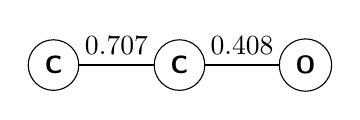
\begin{tikzpicture}[node distance=1.6cm,
  main node/.style={circle,draw,font=\sffamily\small\bfseries}]
  \node[main node] (1) {C};
  \node[main node] (2) [right of=1] {C};
  \node[main node] (3) [right of=2] {O};
  \draw[thick] (1) -- node[above] {$0.707$} (2);
  \draw[thick] (2) -- node[above] {$0.408$} (3);
\end{tikzpicture}
&
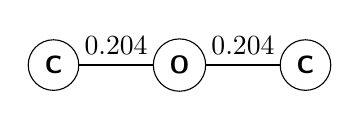
\begin{tikzpicture}[node distance=1.6cm,
  main node/.style={circle,draw,font=\sffamily\small\bfseries}]
  \node[main node] (1) {C};
  \node[main node] (2) [right of=1] {O};
  \node[main node] (3) [right of=2] {C};
  \draw[thick] (1) -- node[above] {$0.204$} (2);
  \draw[thick] (2) -- node[above] {$0.204$} (3);
\end{tikzpicture}\\[4pt]
(a) Ethanol ($\CDZ\approx1.115$) & (b) Dimethyl ether ($\CDZ\approx0.408$)
\end{tabular}
\caption{Edge contributions $\gcdd(a_u,a_v)/\sqrt{a_ua_v}$ for two molecules with
isomorphic hydrogen-suppressed graphs. In (a) the oxygen is terminal
($a_{\mathrm O}=8$), in (b) central ($a_{\mathrm O}=16$).}
\label{fig:isomers}
\end{figure}

\subsubsection*{The scale of the phenomenon}

To determine how general this is we carried out an exhaustive count. For each
$n$ we generated every tree on $n$ vertices, every assignment of the labels
$Z\in\{6,7,8\}$ (carbon, nitrogen, oxygen) to its vertices, and reduced the
result modulo \emph{label-preserving} isomorphism, two structures being
identified only when an isomorphism respecting the atomic numbers exists.
Isomorphism classes were separated using Weisfeiler--Lehman hashing with the
atomic number as the node attribute \cite{shervashidze2011}, with exact
verification within each hash bucket. We then counted how many of the resulting
structures each index separates (Table~\ref{tab:labelled}).

\begin{table}[htbp]
\centering
\caption{Proportion of structures separated -- the number of distinct index
values divided by the number of structures, i.e.\ $1-D(TI)$ in the notation of
\S\ref{sec:degeneracy} -- over all trees labelled by C, N and O. A
vertex-degree-based index ignores the labels, so it takes at most as many
values as there are unlabelled trees on $n$ vertices ($2$, $3$, $6$ and $11$ for
$n=4,\dots,7$). $R$, $GA$, $SO$ and $SDD$ attain this ceiling at every $n$; $ABC$
and $M_2$ attain it for $n\le6$ and take $10$ and $9$ values at $n=7$, which
also rounds to $0.1\%$. $\CDZhom$ attains the same ceiling.}
\label{tab:labelled}
\begin{tabular}{rrccc}
\toprule
$n$ & structures & $\CDZ$ & $\CDZhom$ & classical indices \\
\midrule
$4$ & $75$   & $\mathbf{90.7\%}$ & $2.7\%$ & $2.7\%$ \\
$5$ & $342$  & $\mathbf{82.7\%}$ & $0.9\%$ & $0.9\%$ \\
$6$ & $1773$ & $\mathbf{75.2\%}$ & $0.3\%$ & $0.3\%$ \\
$7$ & $9894$ & $\mathbf{65.3\%}$ & $0.1\%$ & $0.1\%$ \\
\bottomrule
\end{tabular}
\end{table}

The result is categorical. At $n=7$, of $9894$ structures the classical indices
take at most $11$ distinct values -- one per unlabelled tree -- while $\CDZ$
takes $6458$, a factor of about $590$, growing with $n$. The decisive column is
$\CDZhom$: when the atomic numbers are held constant, $\CDZ$'s performance drops
to \emph{exactly} the ceiling attained by the best classical indices. The
advantage therefore comes not from the gcd construction but directly and solely
from the atomic-number weighting, which is the clearest available evidence that
the design intent of the index is realised. We note that
Table~\ref{tab:labelled} is a statement about mathematical separation, obtained
by direct enumeration, and is not subject to sampling or measurement error;
\S\ref{sec:ranking} examines, separately, whether that separation points in the
physically correct direction.

\subsubsection*{Variance explained on measured and computed properties}

To test whether the atomic-number component also carries physicochemical
information we examined five independent heteroatom-containing datasets. Three
(HER2, a large IC$_{50}$ set, and an \textit{E.~coli} set) were assembled from
ChEMBL \cite{chembl2024}; in these the LogP and TPSA values are not measured but
\emph{computed} descriptors, from the Crippen \cite{wildman1999} and Ertl
\cite{ertl2000} algorithms respectively. The remaining two are established public
QSPR benchmarks with \emph{measured} responses: the ESOL set of aqueous
solubilities \cite{delaney2004} and the MoleculeNet Lipophilicity set of LogD
values \cite{wu2018}. The distinction matters: a relation with a computed
descriptor may arise because two algorithms share structural inputs, whereas a
relation with measured data is not subject to that reservation. The ChEMBL sets,
being assembled per biological target, are also likely to contain congeneric
series, which weakens sample independence and may render $p$ values optimistic;
this risk is markedly lower for ESOL and Lipophilicity.

Because every index of this kind grows with molecular size, a raw correlation
would largely measure size. We therefore report the \emph{partial} $R^2$: the
variance in the property explained by the index after the effect of a size
variable (heavy-atom count or molecular weight) has been removed from both.

\begin{table}[htbp]
\centering
\small
\caption{Variance in each property explained by $\CDZ$ after controlling for
molecular size. The size covariate is the heavy-atom count (HAC) or the
molecular weight (MW), as indicated. The $Z$ column uses the true atomic
numbers; the $Z{=}6$ column is the ablation control $\CDZhom$.}
\label{tab:hetero}
\begin{tabular}{llrccc}
\toprule
Dataset & Property & $n$ & size & partial $R^2$ ($Z$) & partial $R^2$ ($Z{=}6$) \\
\midrule
HER2             & LogP (computed)        & $2589$  & HAC & $0.141$ & $0.025$ \\
Large IC$_{50}$  & LogP (computed)        & $10833$ & MW  & $0.097$ & $0.000$ \\
\textit{E.~coli} & LogP (computed)        & $1082$  & HAC & $0.287$ & $0.123$ \\
HER2             & TPSA (computed)        & $2589$  & HAC & $0.194$ & $0.095$ \\
\textit{E.~coli} & TPSA (computed)        & $1082$  & HAC & $0.355$ & $0.162$ \\
ESOL             & solubility (measured)  & $1128$  & MW  & $0.137$ & $0.040$ \\
Lipophilicity    & LogD (measured)        & $4200$  & HAC & $0.019$ & $0.012$ \\
\midrule
Large IC$_{50}$  & molar refractivity     & $10833$ & MW  & $0.271$ & $\mathbf{0.319}$ \\
\textit{E.~coli} & molar volume           & $1082$  & HAC & $0.217$ & $\mathbf{0.292}$ \\
\bottomrule
\end{tabular}
\end{table}

Table~\ref{tab:hetero} shows two distinct patterns. For properties related to
\textbf{polarity} (LogP, TPSA, aqueous solubility, LogD) the true atomic numbers
explain more variance than the homogeneous assumption in \emph{all seven} tests,
and in each the partial $F$-test for adding $\CDZ$ to the size covariate gives
$p<10^{-18}$. (This tests the contribution of $\CDZ$, not the difference between
the two columns, which we do not test formally.) Given that the sample sizes
range from $1082$ to $10\,833$ and the data come from different sources and
targets, the invariance of the direction is a notable consistency. The
\emph{effect size}, by contrast, varies considerably across datasets
($0.019$ to $0.355$); $\CDZ$ should accordingly be regarded not as a strong
predictor on its own but as a complementary descriptor capable of adding
information to an existing model. For \textbf{bulk and refractivity} properties
the pattern reverses and the homogeneous assumption does better, which supports
the interpretation that the atomic-number weighting tracks electron distribution
and polarity rather than molecular size.

\begin{remark}[A retracted finding]
\label{rem:retracted}
On a small dataset ($n=18$) molar refractivity initially appeared to be the
property on which the atomic-number component gained the most (partial $R^2$
$0.189$ against $0.0007$). Repeated on a sample some $600$ times larger, the
comparison \emph{reversed}, as the molar-refractivity row of
Table~\ref{tab:hetero} shows; molar volume, on a second independent set,
behaves in the same way.
We record this as a methodological warning: small-sample findings of this kind
require confirmation on independent large datasets before they are reported as
properties of an index.
\end{remark}

For the smaller aliphatic series the picture is more favourable.
Table~\ref{tab:small} reports single-descriptor models for the normal boiling
point over a set of $45$ aliphatic alcohols, ethers and amines, validated by
leave-one-out cross-validation and by $20$ random $70/30$ external splits; the
external-validation criteria of Golbraikh and Tropsha \cite{golbraikh2002} are
satisfied (mean $R^2_{\mathrm{ext}}=0.673>0.6$, regression-through-origin slopes
$k=1.019$ and $k'=0.910$), and a $Y$-randomisation test over $200$ permutations
gave a mean $R^2$ of $0.022$ and a maximum of $0.252$, well below the observed
value.

\begin{table}[htbp]
\centering
\caption{Single-descriptor models for the normal boiling point, $n=45$.}
\label{tab:small}
\begin{tabular}{lcccc}
\toprule
Descriptor & $R^2$ & $Q^2_{\mathrm{LOO}}$ & RMSE ($^\circ$C) & $R^2_{\mathrm{ext}}$ \\
\midrule
$\CDZ$           & $0.703$ & $0.678$ & $26.35$ & $0.673$ \\
Randi\'c         & $0.590$ & $0.547$ & $30.99$ & --- \\
$ABC$            & $0.516$ & $0.451$ & $33.68$ & --- \\
Heavy-atom count & $0.584$ & $0.538$ & $31.19$ & --- \\
\bottomrule
\end{tabular}
\end{table}

The partial $F$-tests in Table~\ref{tab:partialF} show a one-sided relation on
this set: $\CDZ$ adds significant information to a model containing the Randi\'c
index, whereas the converse does not hold.

\begin{table}[htbp]
\centering
\caption{Partial $F$-tests on the aliphatic set ($n=45$).}
\label{tab:partialF}
\begin{tabular}{lccc}
\toprule
Model extension & $F(1,42)$ & $p$ & adjusted $R^2$ \\
\midrule
Randi\'c $\to$ Randi\'c $+\ \CDZ$ & $16.36$ & $2.2\times10^{-4}$ & $0.580\to0.691$ \\
$ABC$ $\to$ $ABC$ $+\ \CDZ$       & $26.75$ & $6.1\times10^{-6}$ & $0.504\to0.690$ \\
$\CDZ\to\CDZ+$ Randi\'c           & $0.18$  & $0.67$             & $0.697\to0.691$ \\
\bottomrule
\end{tabular}
\end{table}

A triple of isosteric molecules illustrates the mechanism directly. Since $R$
and $ABC$ depend only on the hydrogen-suppressed graph, they assign the
identical values
$1.914$ and $2.121$ to 1-propanol, methyl ethyl ether and propylamine, whose
hydrogen-suppressed graphs are all $P_4$. $\CDZ$ separates them, and on this
triple the separation reproduces the experimental ordering of boiling points:
\[
\begin{array}{lccc}
 & \text{1-propanol} & \text{propylamine} & \text{methyl ethyl ether}\\[2pt]
\CDZ & 2.115 & 1.816 & 1.200\\
\text{b.p.}~(^\circ\mathrm C) & 97.2 & 47.8 & 7.4
\end{array}
\]
The same holds for the 1-butanol / butylamine / diethyl ether triple
($\CDZ$ $3.115$, $2.816$, $1.992$; b.p.\ $117.7$, $77.8$, $34.6\,^\circ$C) and for
the branched pair 2-propanol / isopropylamine ($1.321$ and $1.244$; $82.4$ and
$31.7\,^\circ$C). These are only three examples, chosen because they are the
isosteric groups present in the set; the next subsection tests the agreement
systematically rather than anecdotally.

\subsection{Separating structures versus separating them in the right direction}
\label{sec:ranking}

Table~\ref{tab:labelled} establishes that $\CDZ$ assigns different values to
molecules that differ only in heteroatom placement. A separate question is
whether the \emph{ordering} of those values agrees with the ordering of a
measured property. Being able to separate and being able to separate in the right
direction are distinct claims, and the second does not follow from the first.

We therefore scanned both measured benchmark sets, ESOL and Lipophilicity, for
all \emph{isosteric pairs}: pairs of molecules whose hydrogen-suppressed graphs
are isomorphic as unlabelled graphs. By definition every VDB index assigns both
members of such a pair the same value and so makes no prediction about their
order. For each pair we compared the sign of the difference in $\CDZ$ with the
sign of the difference in the measured property, counting the pair as correctly
ordered when the signs agree. Filtering out pairs of differing composition (for
instance one chlorinated and one brominated molecule) leaves only \emph{true
positional isomers}: pairs with the same molecular formula differing solely in
heteroatom placement -- the general form of the ethanol / dimethyl ether example,
and the real target of the test. Results are in Table~\ref{tab:ranking}.

\begin{table}[htbp]
\centering
\caption{Agreement between the $\CDZ$ ordering and the measured-property ordering
on isosteric pairs, with two-sided binomial $p$ values against $50\%$. The
middle rows contain only true positional isomers, i.e.\ pairs with identical
molecular formula (hydrogens included); the last rows use the looser criterion
of an identical multiset of heavy atoms, with the hydrogen count not compared.}
\label{tab:ranking}
\begin{tabular}{llrcc}
\toprule
Dataset & Pair type & $n$ & correctly ordered & $p$ \\
\midrule
ESOL          & all isosteric pairs     & $2124$ & $42.8\%$ & $3\times10^{-11}$ \\
Lipophilicity & all isosteric pairs     & $1073$ & $55.7\%$ & $2\times10^{-4}$ \\
\midrule
ESOL          & true positional isomers & $50$   & $54.0\%$ & $0.67$ \\
Lipophilicity & true positional isomers & $82$   & $52.4\%$ & $0.74$ \\
\midrule
ESOL          & same heavy atoms        & $81$   & $56.8\%$ & $0.27$ \\
Lipophilicity & same heavy atoms        & $89$   & $53.9\%$ & $0.53$ \\
\bottomrule
\end{tabular}
\end{table}

The outcome does not favour $\CDZ$, and is recorded as it stands.

On true positional isomers ($n=50$ and $n=82$) the agreement rates of $54.0\%$
and $52.4\%$ are statistically indistinguishable from chance ($p=0.67$ and
$p=0.74$), and the same holds under the looser heavy-atom criterion ($56.8\%$
and $53.9\%$, $p=0.27$ and $p=0.53$). The ordering $\CDZ$ assigns to isosteric pairs therefore does not
agree significantly with the ordering of measured solubility or LogD.

The small $p$ values in the first two rows are misleading and should be
interpreted with care. The large majority of those pairs are not positional
isomers but molecules sharing only a graph shape while differing in composition;
that $\CDZ$ distinguishes these is expected and does not test the index's actual
claim. Moreover the two datasets point in opposite directions: in ESOL the rate
is \emph{below} $50\%$ ($42.8\%$), meaning $\CDZ$ systematically inverts the
solubility ordering, while in Lipophilicity it is above. With no consistent
direction, no general rule can be drawn from these two rows.

This finding does not invalidate Table~\ref{tab:labelled}, but it does bound its
scope. That $\CDZ$ discriminates heteroatom placement is an exact mathematical
fact. That the discrimination is physicochemically correctly oriented is
\emph{not} supported by the measured data available to us. Converting the
index's structural discriminating power into predictive power will likely require
using $\CDZ$ not alone but as one component of a suitable descriptor set.

%%%%%%%%%%%%%%%%%%%%%%%%%%%%%%%%%%%%%%%%%%%%%%%%%%%%%%%%%%%%%%%%%%%%%%%%%%%%%
\section{Limitations and applicability domain}
\label{sec:limits}

A complete account requires reporting where the index does \emph{not} perform
well.

\begin{enumerate}
\item \textbf{Pure-carbon systems.} By Proposition~\ref{prop:homog} the
      atomic-number component cancels identically on hydrocarbon skeletons, so on
      the octane isomers (Table~\ref{tab:octane}) and on benzenoid series $\CDZ$
      reduces to $\CDZhom$ and is outperformed by the classical indices on five
      of the six properties tested. Reported
      correlations for such series should be read with this in mind: on linear
      acenes, for instance, a very high correlation with total $\pi$-electron
      energy is obtained, but the edge count $m$ alone attains the same value,
      because in that series every quantity involved is linear in the number of
      rings.
\item \textbf{Carbon-rich aromatic systems.} On the large IC$_{50}$ set ($10\,833$ ligands)
      the one-sided relation of Table~\ref{tab:partialF} reverses. Taking molar
      refractivity as the response, $\CDZ$ attains $Q^2=0.792$ against $0.969$
      for the Randi\'c index, $0.961$ for $ABC$ and $0.967$ for the heavy-atom
      count; adding Randi\'c to a model containing $\CDZ$ raises $R^2$ from
      $0.792$ to $0.969$, whereas adding $\CDZ$ to a model containing Randi\'c
      leaves $R^2$ unchanged to four decimal places (the partial $F$-test is
      nominally significant at $p=0.026$, an artefact of the sample size).
      The gap persists after controlling for size: with the heavy-atom count
      partialled out, $\CDZ$ explains $0.8\%$ of the remaining variance in molar
      refractivity and Randi\'c $5.4\%$, and within strata of equal heavy-atom
      count (those with at least $100$ molecules) Randi\'c explains more of the
      variance than $\CDZ$ in $19$ of $28$.
\item \textbf{Abrupt response to structural change.} The non-monotonicity of
      Remark~\ref{rem:nonmonotone} has the measurable consequence quantified in
      \S\ref{sec:ssabr}: $\CDZ$ has the lowest or second-lowest $SS/Abr$ ratio
      of the twelve indices at every order tested. The index responds sharply
      rather than smoothly to local modification -- an advantage for
      discrimination, a disadvantage for interpolating properties across a
      homologous series.
\item \textbf{Direction of discrimination.} As \S\ref{sec:ranking} reports, the
      ordering $\CDZ$ induces on true positional isomers is not significantly
      better than chance against measured solubility and LogD.
\item \textbf{Branching.} The index does not reliably order branched isomers
      within a homologous series.
\item \textbf{Bond order.} Definition~\ref{def:cdz} uses the heavy-atom degree
      and ignores bond multiplicity, so benzene and cyclohexane receive equal
      values.
\item \textbf{Biological activity.} On the same set no two-dimensional
      topological index -- $\CDZ$, Randi\'c, $ABC$ or heavy-atom count --
      predicted $\mathrm{pIC}_{50}$ ($Q^2\le0.073$ throughout). This reflects a
      general limitation of connectivity descriptors rather than a property of
      $\CDZ$.
\item \textbf{Open extremal problem.} No proof of Conjecture~\ref{conj:min} is
      available, hence no closed-form characterisation of the minimising trees
      and no sharp lower bound over chemical trees
      (Remark~\ref{rem:chemical_gap}).
\end{enumerate}

Accordingly the applicability domain of $\CDZ$ is best described as small to
medium-sized, predominantly aliphatic molecules with varied heteroatom
environments, used as a complementary descriptor rather than a stand-alone
predictor.

\begin{remark}[Generalisation to other vertex invariants]
\label{rem:generalisation}
The construction uses the immediate valence $d_u$, but the algebraic framework
extends to any strictly positive vertex invariant $w_u$ via $a_u=w_uZ_u$. Two
natural choices are the eccentricity $w_u=\varepsilon(u)$, which captures
long-range topological effects, and $w_u=\sum_{v\in N(u)}d_v$, which captures
steric crowding. All such variants inherit the isomorphism invariance of
Remark~\ref{rem:isom}, since both $\varepsilon(u)$ and $\sum_{v\in N(u)}d_v$ are
themselves isomorphism-invariant vertex statistics. None of the extremal results
of Sections~\ref{sec:bounds}--\ref{sec:classes} is established for these
generalised weights, and they are mentioned here only as directions for further
work.
\end{remark}

%%%%%%%%%%%%%%%%%%%%%%%%%%%%%%%%%%%%%%%%%%%%%%%%%%%%%%%%%%%%%%%%%%%%%%%%%%%%%
\section{Conclusion}
\label{sec:conclusion}

The index $\CDZ$ is well defined, invariant under isomorphism of labelled
molecular graphs, computable in essentially linear time, and admits a complete
extremal theory on trees: $\sqrt{n-1}\le\CDZ(T)\le n-3+\sqrt2$ with the star and
the path as the unique extremal graphs, together with closed forms on the
standard families and exact two-sided comparisons with the Randi\'c and
geometric-arithmetic indices whose equality cases are characterised -- the
Randi\'c one by the arithmetic condition that adjacent degrees be coprime, a type
of characterisation we are not aware of elsewhere in this literature.

Empirically the assessment separates cleanly into two regimes, and the separation
is explained by a single structural fact, the homogeneous reduction of
Proposition~\ref{prop:homog}. On pure-carbon testbeds $\CDZ$ collapses to a
degree-based invariant: there it matches the best classical indices in
discriminative power while remaining uncorrelated with all of them -- its
correlations lie below the weakest of the $55$ mutual correlations among the
eleven comparison indices -- but it is outperformed by them on five of the six
thermodynamic properties tested. Where heteroatoms are present the atomic-number
component becomes active and the gain is categorical rather than marginal: over
all trees on seven vertices labelled by C, N and O it separates $65.3\%$ of the
$9894$ structures against $0.1\%$ for every classical index, and the $\CDZhom$
ablation shows that this entire advantage is attributable to the atomic numbers.

Equally, the limits are explicit. The separation of isosteric structures is an
exact mathematical fact; its physicochemical orientation is not supported by the
measured solubility and LogD data examined here, where the ordering of true
positional isomers is indistinguishable from chance. The index also responds
abruptly rather than smoothly to local structural change, a direct consequence of
the discontinuity of the gcd. Taken together, these results position $\CDZ$ as a
structural discriminator and complementary descriptor rather than a stand-alone
predictor.

On the extremal side, the minimisers over chemical trees on up to $17$ vertices
are either members of an explicit two-parameter family or, at the four orders
where a vertex of degree two appears, are explained by the subdivision identity
of Lemma~\ref{lem:subdiv}; that identity also shows that the minimiser on $n$
vertices need not arise from the minimiser on $n-1$, since subdividing an edge
of type $(3,3)$ is the only subdivision that lowers the index.

The principal open questions are Conjecture~\ref{conj:min}, which splits into a
case that yields, for edges of type $(3,3)$, to the local analysis of
\S\ref{sec:local} and Appendix~\ref{app:local} -- reduced by
Problem~\ref{prob:partial} to a purely existential statement, with the $(4,4)$
case still needing further configurations -- and a residual case $d_u=d_v=2$ for
which Remark~\ref{rem:obstruction} shows that strict descent by single-edge
moves does not suffice, and which Problem~\ref{prob:global} refines; Conjecture~\ref{conj:unicyclic} on the unicyclic minimisers; and the
sharp lower bound over chemical trees, which Remark~\ref{rem:chemical_gap} shows
is not supplied by the unrestricted bound.

%%%%%%%%%%%%%%%%%%%%%%%%%%%%%%%%%%%%%%%%%%%%%%%%%%%%%%%%%%%%%%%%%%%%%%%%%%%%%
\section*{Data and code availability}

All graph enumerations and index computations reported here were carried out
with Python scripts using \texttt{networkx} \cite{hagberg2008}, \texttt{numpy}
and \texttt{scipy}. The scripts, the datasets in the form used, and a driver
that runs every script and checks its output against the values printed in this
paper are openly available on GitHub and archived at Zenodo,
\url{https://doi.org/10.5281/zenodo.24505775}. Each table,
proposition verified by computation, and remark resting on a search is mapped to
the script that reproduces it in the repository's \texttt{README}. Molecular
graphs are read from SMILES by a parser included in the repository, which agrees
with an RDKit-based computation \cite{rdkit} of $\CDZ$ on all $10\,833$ molecules
of the largest set; the physicochemical descriptors supplied with the ChEMBL
sets (molecular weight, LogP, TPSA, molar refractivity) were computed with RDKit.
The ESOL \cite{delaney2004} and Lipophilicity \cite{wu2018} datasets are public;
the three ChEMBL-derived sets \cite{chembl2024} were filtered for single-protein
targets with reported IC$_{50}$ or EC$_{50}$ values and standardised before use.
Octane boiling points and enthalpies were checked against the NIST Chemistry
WebBook \cite{nist}.

%%%%%%%%%%%%%%%%%%%%%%%%%%%%%%%%%%%%%%%%%%%%%%%%%%%%%%%%%%%%%%%%%%%%%%%%%%%%%%%%%%%%%%%%%%%%%%%%%%%%%%%%%%%%%%%%%%%%%%%%%%%%%%%%%%%%%%%%%%%%%%%%%%
\appendix
\section{The local analysis behind Proposition~\ref{prop:partialres}}
\label{app:local}

We prove part~(a) of Proposition~\ref{prop:partialres}, keeping the notation
$w(a,b)=\gcdd(a,b)/\sqrt{ab}$ of \S\ref{sec:subdivision}.

\subsection*{The local formula}

\begin{lemma}[Effect of a leaf relocation]
\label{lem:local}
Let $x$ be a leaf of $T$ with neighbour $p$, and let $t\notin\{x,p\}$ satisfy
$d_t\le3$. Let $T'$ be obtained from $T$ by deleting $px$ and adding $tx$. If
$t\notin N(p)$, then
\[
  \CDZ(T')-\CDZ(T)\;=\;A(p,x)+B(t),
\]
where
\begin{align*}
  A(p,x)&=-w(d_p,1)+\sum_{y\in N(p)\setminus\{x\}}
         \bigl[w(d_p-1,d_y)-w(d_p,d_y)\bigr],\\
  B(t)&=w(d_t+1,1)+\sum_{z\in N(t)}
         \bigl[w(d_t+1,d_z)-w(d_t,d_z)\bigr].
\end{align*}
If $t\in N(p)$, the same expression holds once the term for $y=t$ is omitted from
$A$, the term for $z=p$ is omitted from $B$, and $w(d_p-1,d_t+1)-w(d_p,d_t)$ is
added.
\end{lemma}

\begin{proof}
Only the edges incident with $p$, with $t$, and the relocated edge itself change
their contribution; every other edge joins two vertices whose degrees are
unaffected. Collecting terms gives the identity, the second form accounting for
the edge $pt$, whose contribution changes at both ends.
\end{proof}

Thus $A$ measures the gain from detaching a leaf at $p$ and $B$ the cost of
attaching one at $t$; both depend only on the degrees of $p$, of $t$ and of their
neighbours, so each is determined by a finite table.

\subsection*{Donors}

\begin{lemma}[Degree-two donor]
\label{lem:donorA}
Let $n\ge4$ and let $p$ be a vertex of $T$ with $d_p=2$ having a leaf neighbour
$x$. Then $A(p,x)\le-0.53800$.
\end{lemma}

\begin{proof}
Let $c$ be the degree of the other neighbour of $p$. Then
$A(p,x)=-w(2,1)+w(1,c)-w(2,c)$, giving $-0.41421$, $-1.00000$, $-0.53800$ and
$-0.91421$ for $c=1,2,3,4$ respectively. The value $c=1$ forces $p$ together
with its two leaf neighbours to be the whole tree, i.e.\ $T\cong P_3$, excluded
by $n\ge4$. The maximum of the remaining three values is $-0.53800$.
\end{proof}

\begin{lemma}[Donor at a $(3,3)$ edge]
\label{lem:donorE}
Let $uv$ be an edge with $d_u=d_v=3$ and let $x$ be a leaf neighbour of $u$.
Then $A(u,x)\le-0.57735$.
\end{lemma}

\begin{proof}
Write $m'(c)=w(2,c)-w(3,c)$, so $m'(1)=0.12976$, $m'(2)=0.59175$,
$m'(3)=-0.59175$ and $m'(4)=0.41843$. If $c$ is the degree of the third
neighbour of $u$, then, using $d_v=3$,
\[
  A(u,x)=-w(3,1)+m'(3)+m'(c)=-1.16910+m'(c),
\]
which equals $-1.03935$, $-0.57735$, $-1.76085$ and $-0.75067$ for $c=1,2,3,4$.
All four are negative; the maximum is $-0.57735$.
\end{proof}

The mechanism is worth recording: the presence of the $(3,3)$ edge itself
supplies the term $m'(3)=-0.59175$, so a $(3,3)$ edge guarantees its own donor
bound. No analogous unconditional statement holds at a $(4,4)$ edge.

\begin{lemma}[Donor at a $(4,4)$ edge]
\label{lem:donorC}
Let $uv$ be an edge with $d_u=d_v=4$, let $x$ be a leaf neighbour of $u$, and let
$a,b$ be the degrees of the two remaining neighbours of $u$. Then
$A(u,x)=-1.21132+h(a)+h(b)$ with $h(d)=w(3,d)-w(4,d)$, and $A(u,x)\le-0.42265$
unless $\{a,b\}=\{3,3\}$, in which case $A(u,x)=+0.21132$.
\end{lemma}

\begin{proof}
Here $h(1)=0.07735$, $h(2)=-0.29886$, $h(3)=0.71132$ and $h(4)=-0.71132$, and
$d_v=4$ contributes $h(4)$. Evaluating $-0.5+h(4)+h(a)+h(b)$ over the ten
unordered pairs $\{a,b\}$ gives $-1.05662$, $-1.43283$, $-0.42265$, $-1.84530$,
$-1.80904$, $-0.79886$, $-2.22151$, $+0.21132$, $-1.21132$ and $-2.63397$ for
$(1,1),(1,2),(1,3),(1,4),(2,2),(2,3),(2,4),(3,3),(3,4),(4,4)$.
\end{proof}

The single failure $\{a,b\}=\{3,3\}$ is exactly the phenomenon anticipated above:
lowering $d_u$ from $4$ to $3$ creates a new $(3,3)$ edge at each degree-$3$
neighbour, and such an edge contributes the maximal value $1$.

\subsection*{Recipients}

\begin{lemma}[Recipients]
\label{lem:recipients}
\begin{enumerate}
\item If $t$ is a leaf whose neighbour has degree $3$, then $B(t)=0.53800$.
\item If $d_u=3$ and $uv$ is a $(3,3)$ edge, and $a,b$ are the degrees of the
      other two neighbours of $u$, then $B(u)=-0.21132+g(a)+g(b)$ with
      $g(d)=w(4,d)-w(3,d)$.
\item If $d_u=4$ and $t\in N(u)$ has $d_t=2$ with other neighbour of degree $c$,
      then $B(t)=0.15892+m(c)$ with $m(d)=w(3,d)-w(2,d)$, giving $0.02916$,
      $-0.43283$, $0.75067$ and $-0.25951$ for $c=1,2,3,4$.
\end{enumerate}
\end{lemma}

\begin{proof}
Direct evaluation of $B$ in Lemma~\ref{lem:local}; in (ii) the term for $v$
contributes $g(3)=-0.71132$, and in (iii) the term for $u$ contributes
$m(4)=-0.41843$.
\end{proof}

\subsection*{The cases}

\begin{proposition}[Case 1]
\label{prop:case1}
Let $uv$ be a $(3,3)$ edge and suppose $T$ has a vertex $p$ with $d_p=2$ carrying
a leaf $x$, with $p\ne u$ and $x\ne u$. Let $a,b$ be the degrees of the two
neighbours of $u$ other than $v$. If
$\{a,b\}\notin\bigl\{\{2,4\},\{4,4\}\bigr\}$, then moving $x$ to $u$ strictly
decreases $\CDZ$.
\end{proposition}

\begin{proof}
By Lemmas~\ref{lem:donorA} and~\ref{lem:recipients}(ii) the change is at most
$-0.53800+B(u)$. Evaluating $B(u)$ over the ten pairs gives $-0.36603$,
$0.01018$, $-1.00000$, $0.42265$, $0.38639$, $-0.62379$, $0.79886$, $-1.63397$,
$-0.21132$ and $1.21132$ in the order listed in Lemma~\ref{lem:donorC}; adding
$-0.53800$ leaves a negative total in all cases except $\{2,4\}$ and $\{4,4\}$.
\end{proof}

Two margins here are slender: $-0.11535$ for $\{a,b\}=\{1,4\}$ and $-0.15161$ for
$\{a,b\}=\{2,2\}$. Both would fail under the weaker bound $A\le-0.41421$, so the
exclusion of $T\cong P_3$ in Lemma~\ref{lem:donorA} is doing real work.

\begin{proposition}[Case 2]
\label{prop:case2}
Let $uv$ be a $(3,3)$ edge, let $x$ be a leaf neighbour of $u$, and let $t\ne x$
be a leaf whose neighbour has degree $3$. Then moving $x$ to $t$ strictly
decreases $\CDZ$, by at least $0.03935$.
\end{proposition}

\begin{proof}
If $t$ is not adjacent to $u$, Lemmas~\ref{lem:donorE}
and~\ref{lem:recipients}(i) give a change of at most
$-0.57735+0.53800=-0.03935$.

If $t$ is adjacent to $u$, then the degree-$3$ neighbour of $t$ is $u$ itself, so
$t$ is a second leaf of $u$ and, since $d_u=3$, the neighbours of $u$ are exactly
$v$, $x$ and $t$. The adjacent form of Lemma~\ref{lem:local} then gives
\begin{align*}
  &\bigl[-w(3,1)+w(2,1)\bigr]+\bigl[w(2,3)-w(3,3)\bigr]+\bigl[w(2,2)-w(3,1)\bigr]\\
  &\qquad=\;0.12976-0.59175+0.42265\;=\;-0.03935,
\end{align*}
the same value.
\end{proof}

\begin{proposition}[Case 3]
\label{prop:case3}
Let $uv$ be a $(4,4)$ edge, let $p\ne t$ be a vertex with $d_p=2$ carrying a leaf
$x$, and let $t\in N(u)$ with $d_t=2$ whose other neighbour has degree $c\ne3$.
Then moving $x$ to $t$ strictly decreases $\CDZ$.
\end{proposition}

\begin{proof}
By Lemmas~\ref{lem:donorA} and~\ref{lem:recipients}(iii) the change is at most
$-0.53800+B(t)$, equal to $-0.50884$, $-0.97083$ and $-0.79751$ for $c=1,2,4$.
\end{proof}

\begin{proposition}[Case 4]
\label{prop:case4}
Let $uv$ be a $(3,3)$ edge, let $p\in N(u)$ with $d_p=4$, let $x$ be a leaf
neighbour of $p$, let $e_1,e_2$ be the degrees of the neighbours of $p$ other
than $u$ and $x$, and let $c$ be the degree of the neighbour of $u$ other than
$v$ and $p$. Then moving $x$ to $u$ changes $\CDZ$ by exactly
\[
  h(e_1)+h(e_2)+g(3)+g(c)\;=\;h(e_1)+h(e_2)-0.71132+g(c),
\]
which is negative for $29$ of the $40$ profiles $(\{e_1,e_2\},c)$.
\end{proposition}

\begin{proof}
Here $d_p$ drops from $4$ to $3$ and $d_u$ rises from $3$ to $4$, and $p,u$ are
adjacent. In the adjacent form of Lemma~\ref{lem:local} the relocated edge
contributes $-w(4,1)+w(4,1)=0$ and the adjacency correction
$w(3,4)-w(4,3)=0$; the remaining terms are those displayed, the term $g(3)$
coming from $v$.
\end{proof}

\begin{proposition}[Case 5]
\label{prop:case5}
Let $uv$ be a $(3,3)$ edge, let $x$ be a leaf neighbour of $v$, and let
$t\in N(v)$ with $d_t=2$, so that $N(v)=\{u,x,t\}$. Let $c$ be the degree of the
neighbour of $t$ other than $v$. Then moving $x$ to $t$ changes $\CDZ$ by exactly
$-0.59175+m(c)$, which equals $-0.72151$, $-1.18350$, $0$ and $-1.01018$ for
$c=1,2,3,4$; in particular the move strictly decreases $\CDZ$ whenever $c\ne3$.
\end{proposition}

\begin{proof}
Again $p=v$ and $t$ are adjacent. The relocated edge contributes
$-w(3,1)+w(3,1)=0$ and the adjacency correction $w(2,3)-w(3,2)=0$; what remains
is the term $w(2,3)-w(3,3)=-0.59175$ from $u$ and the term $m(c)$ from the other
neighbour of $t$.
\end{proof}

\subsection*{Status of the argument}

Over the $10\,818$ chemical trees with $5\le n\le16$ containing an edge $uv$
with $d_u=d_v\ge3$, the five configurations, each evaluated by direct
computation of $\CDZ$ on the relocated tree, cover $10\,445$. They cover
\emph{every} one of the $8903$ trees that contain a $(3,3)$ edge; the $373$ trees
left uncovered all have $(4,4)$ edges as their only equal-degree edges, so
Case~3 and Lemma~\ref{lem:donorC} do not by themselves dispose of the $(4,4)$
case. Each of those $373$ trees nevertheless admits an improving leaf
relocation, found by exhaustive search over moves; in no instance is a branch
relocation needed.

The five propositions and the five lemmas supporting them are complete proofs:
each is a finite evaluation over degree profiles, and each exhibits an explicit
move together with an exact value for the resulting change. What remains is
purely existential -- that the donors and recipients they require are always
present -- and this has so far been established only computationally, for
$n\le16$ and edges of type $(3,3)$.

We note that the constant $B(t)=0.53800$ of Lemma~\ref{lem:recipients}(i)
equals $\sigma(1,3)$ of~\eqref{eq:sigma}. This is no coincidence: attaching a
new leaf to a leaf $t$ whose neighbour has degree $3$ turns $t$ into a vertex of
degree $2$ on a path from that neighbour to the new leaf, which is the same tree
as subdividing a pendant edge of type $(1,3)$.

%%%%%%%%
\begin{thebibliography}{99}

\bibitem{bollobas1998}
B. Bollob\'as and P. Erd\H{o}s, Graphs of extremal weights,
\emph{Ars Combin.} \textbf{50} (1998) 225--233.

\bibitem{chembl2024}
B. Zdrazil et al., The ChEMBL Database in 2023: a drug discovery platform
spanning multiple bioactivity data types and time periods,
\emph{Nucleic Acids Res.} \textbf{52} (2024) D1180--D1192.

\bibitem{delaney2004}
J. S. Delaney, ESOL: Estimating aqueous solubility directly from molecular
structure, \emph{J. Chem. Inf. Comput. Sci.} \textbf{44} (2004) 1000--1005.

\bibitem{ertl2000}
P. Ertl, B. Rohde and P. Selzer, Fast calculation of molecular polar surface area
as a sum of fragment-based contributions and its application to the prediction of
drug transport properties, \emph{J. Med. Chem.} \textbf{43} (2000) 3714--3717.

\bibitem{estrada1998}
E. Estrada, L. Torres, L. Rodr\'iguez and I. Gutman, An atom-bond connectivity
index: modelling the enthalpy of formation of alkanes,
\emph{Indian J. Chem.} \textbf{37A} (1998) 849--855.

\bibitem{furtula2013}
B. Furtula, I. Gutman and M. Dehmer, On structure-sensitivity of degree-based
topological indices, \emph{Appl. Math. Comput.} \textbf{219} (2013) 8973--8978.

\bibitem{furtula2025}
B. Furtula and M. S. \"Oz, Complementary topological indices,
\emph{MATCH Commun. Math. Comput. Chem.} \textbf{93} (2025) 247--263.

\bibitem{furtula2025ijmc}
B. Furtula and M. S. \"Oz, Geometric-quadratic index from a mathematical
perspective, \emph{Iranian J. Math. Chem.} \textbf{16} (2025) 85--92.

\bibitem{golbraikh2002}
A. Golbraikh and A. Tropsha, Beware of $q^2$!,
\emph{J. Mol. Graph. Model.} \textbf{20} (2002) 269--276.

\bibitem{gutman1972}
I. Gutman and N. Trinajsti\'c, Graph theory and molecular orbitals. Total
$\pi$-electron energy of alternant hydrocarbons,
\emph{Chem. Phys. Lett.} \textbf{17} (1972) 535--538.

\bibitem{gutman1975}
I. Gutman, B. Ru\v{s}\v{c}i\'c, N. Trinajsti\'c and C. F. Wilcox, Graph theory
and molecular orbitals. XII. Acyclic polyenes,
\emph{J. Chem. Phys.} \textbf{62} (1975) 3399--3405.

\bibitem{gutman2013}
I. Gutman, Degree-based topological indices,
\emph{Croat. Chem. Acta} \textbf{86} (2013) 351--361.

\bibitem{gutman2021}
I. Gutman, Geometric approach to degree-based topological indices: Sombor
indices, \emph{MATCH Commun. Math. Comput. Chem.} \textbf{86} (2021) 11--16.

\bibitem{gutman2024}
I. Gutman, B. Furtula and M. S. \"Oz, Geometric approach to vertex-degree-based
topological indices -- Elliptic Sombor index, theory and application,
\emph{Int. J. Quantum Chem.} \textbf{124} (2024) e27346.

\bibitem{hagberg2008}
A. A. Hagberg, D. A. Schult and P. J. Swart, Exploring network structure,
dynamics, and function using NetworkX, in: \emph{Proceedings of the 7th Python in
Science Conference (SciPy 2008)}, Pasadena, 2008, pp.\ 11--15.

\bibitem{konstantinova1996}
E. V. Konstantinova, The discrimination ability of some topological and
information distance indices for graphs of unbranched hexagonal systems,
\emph{J. Chem. Inf. Comput. Sci.} \textbf{36} (1996) 54--57.

\bibitem{kulli2022}
V. R. Kulli, Geometric-quadratic and quadratic-geometric indices,
\emph{Ann. Pure Appl. Math.} \textbf{25} (2022) 1--5.

\bibitem{kumar2024}
V. Kumar and S. Das, On structure sensitivity and chemical applicability of some
novel degree-based topological indices,
\emph{MATCH Commun. Math. Comput. Chem.} \textbf{92} (2024) 165--203.

\bibitem{liu2022}
H. Liu, I. Gutman, L. You and Y. Huang, Sombor index: review of extremal results
and bounds, \emph{J. Math. Chem.} \textbf{60} (2022) 771--798.

\bibitem{nist}
P. J. Linstrom and W. G. Mallard (Eds.), \emph{NIST Chemistry WebBook, NIST
Standard Reference Database Number 69}, National Institute of Standards and
Technology, Gaithersburg MD, \texttt{https://webbook.nist.gov/chemistry/}
(retrieved 24 October 2026).

\bibitem{oz2025}
M. S. \"Oz and I. Gutman, More geometric studies of vertex-degree-based graph
indices -- tangent Sombor index,
\emph{Hacet. J. Math. Stat.} \textbf{54} (2025) 2195--2205.

\bibitem{randic1975}
M. Randi\'c, On characterization of molecular branching,
\emph{J. Am. Chem. Soc.} \textbf{97} (1975) 6609--6615.

\bibitem{rdkit}
G. Landrum et al., RDKit: Open-source cheminformatics,
\texttt{https://www.rdkit.org}.

\bibitem{shervashidze2011}
N. Shervashidze, P. Schweitzer, E. J. van Leeuwen, K. Mehlhorn and
K. M. Borgwardt, Weisfeiler--Lehman graph kernels,
\emph{J. Mach. Learn. Res.} \textbf{12} (2011) 2539--2561.

\bibitem{todeschini2009}
R. Todeschini and V. Consonni, \emph{Molecular Descriptors for
Chemoinformatics}, Wiley-VCH, Weinheim, 2009.

\bibitem{vukicevic2009}
D. Vuki\v{c}evi\'c and B. Furtula, Topological index based on the ratios of
geometrical and arithmetical means of end-vertex degrees of edges,
\emph{J. Math. Chem.} \textbf{46} (2009) 1369--1376.

\bibitem{vukicevic2010}
D. Vuki\v{c}evi\'c and M. Ga\v{s}perov, Bond additive modeling 1. Adriatic
indices, \emph{Croat. Chem. Acta} \textbf{83} (2010) 243--260.

\bibitem{wildman1999}
S. A. Wildman and G. M. Crippen, Prediction of physicochemical parameters by
atomic contributions, \emph{J. Chem. Inf. Comput. Sci.} \textbf{39} (1999)
868--873.

\bibitem{wu2018}
Z. Wu, B. Ramsundar, E. N. Feinberg, J. Gomes, C. Geniesse, A. S. Pappu,
K. Leswing and V. Pande, MoleculeNet: a benchmark for molecular machine learning,
\emph{Chem. Sci.} \textbf{9} (2018) 513--530.

\bibitem{zhou2009}
B. Zhou and N. Trinajsti\'c, On a novel connectivity index,
\emph{J. Math. Chem.} \textbf{46} (2009) 1252--1270.

\end{thebibliography}

\end{document}
